\chapter{Multiple Step Ahead Forecasts of the Disturbance Storm Time Index: The GPNN Model}\label{chapter:dst_msa}

{\small
	We present a method that combines a \emph{long short-term memory} (LSTM) network with a 
	Gaussian process (GP) model to provide up to six-hour-ahead probabilistic forecasts of the Dst 
	geomagnetic index. The proposed approach brings together the sequence modeling capabilities of 
	a recurrent neural network with the error bars and confidence bounds provided by a GP. Our 
	model is trained using the hourly OMNI and Global Positioning System (GPS) databases - both of 
	which are publicly available. We first develop a LSTM network to get a single-point prediction 
	of Dst. This model yields great accuracy in forecasting the Dst index from one to six hours 
	ahead, with a correlation coefficient always higher than $0.873$ and a root mean square error 
	lower than $\SI{9.86}{\nano\tesla}$. However, even if its averaged metrics show excellent 
	performance, it remains poor in predicting superstorms 
	($\mathrm{Dst} < \SI{-250}{\nano\tesla}$) six hours in advance. Next, we combine the LSTM model 
	obtained from the first step with a GP model to yield a hybrid probabilistic predictor and 
	evaluate it using the receiver operating characteristic curve and the reliability diagram. We 
	conclude that this hybrid methodology provides improvements in the forecasting of 
	$\mathrm{Dst}$ from one to five hours ahead.

}
	

\vfill
\sectionlinetwo{DarkGreen}{88}
\vfill

\noindent
	\parbox{\textwidth}{%
		{\small This chapter is based on the following:\\

		\textbf{Article}:\\
		\bibentry{doi:10.1029/2018SW001898}}
    }%

\clearpage

\section{Introduction}

It is widely accepted that solar wind magnetosphere coupling plays a key role in determining the 
Earth’s geomagnetic state. Under appropriate conditions, this coupling can lead to injection of 
energetic particles into the Earth’s auroral and equatorial plasma currents, leading to geomagnetic 
storms. The solar wind conditions that are effective for creating geomagnetic storms are sustained 
periods of high-speed solar wind and a southward directed solar wind magnetic field 
\citep{JGR:JGR10260}. When \citet{1981AkasofuE} studied the coupling function between the solar 
wind and geomagnetic disturbances, they observed that during these extreme events, the key process 
is magnetic reconnection \citep{magneticreconnection}. Magnetic reconnection produces an 
enhancement of particle flux which creates a depression of the horizontal component of the Earth’s 
magnetic field and an intensification of the westward ring current circulating the Earth 
\citep{JGRA:JGRA11775}. When there is a geomagnetic storm, the energy content of the ring current 
increases. This increase is inversely proportional to the strength of the surface magnetic field at 
low latitudes. To assess the severity of geomagnetic storms, the Disturbance Storm Time index 
($Dst$) is often used. 

The Dst index \citep{Sugiura1964} is based on measurements from four low latitude stations and 
represents the axis-symmetric magnetic signature of magnetosphere currents (such as the ring current, 
the tail currents, and the Chapman-Ferraro current). It is computed using $1$-hour average values of the 
horizontal component of the Earth’s magnetic field and is expressed in nano Tesla (nT). In the case of a 
typical magnetic storm, three phases are observed according to Dst variations. First, there is a sudden drop 
corresponding to the storm commencement. Second, the value of Dst stays in its excited state as the ring current 
intensifies (the main phase). Finally, once the $z$-component of the interplanetary magnetic field (IMF) turns 
northward, the ring current begins to recover and rises back to its quiet level (recovery phase). 

Geomagnetic indices like Dst, Kp, AE and others are used in space weather to describe effects of the solar wind on 
the Earth's magnetosphere. It has been long observed that strong geomagnetic storms disrupt man-made systems, 
they can impact satellites, disrupt navigation systems and create harmful geomagnetic induced currents in power grids 
and pipelines. One of the important research problems in space weather is to predict geomagnetic disturbances 
in order to protect technological infrastructure \citep{Singh2010}. The aim of this study is to propose an 
accurate and reliable probabilistic model to predict Dst from one hour to six hours ahead. 

The Dst prediction problem has been extensively researched. \citet{JGR:JGR10260} developed a model 
that expressed the time evolution of Dst as an Ordinary Differential Equation (ODE). This method takes into account 
the particle injection from the plasma sheet into the magnetosphere and expresses it based on the solar wind speed, 
density and on the north-south magnetic component of the IMF ($B_z$). \citet{Iyemori1979} used a linear filtering 
prediction method to connect Dst with the southward component of the interplanetary magnetic field. The linear 
assumption, however, has limitations since the solar wind and the magnetosphere form a coupled non-linear system. 

To model nonlinear behavior of magnetospheric response, various models have been proposed. A popular approach 
used to model nonlinear systems is based on artificial neural networks (ANN) \citep{haykin1994neural}. One of the 
earliest models of Dst prediction based on ANNs is due to \citet{lundstedt1994prediction}. They developed 
a feedforward neural network to predict Dst one hour ahead, using $B_z$, the density, and the velocity of 
the solar wind. This model was able to model the initial and main phases of geomagnetic storms well, but 
the recovery phase was not modeled accurately. \citet{gleisner1996predicting} developed a time delay 
neural network \citep{Waibel1989} to predict Dst one hour ahead using the proton density, solar wind 
velocity, and $Bz$. This approach managed to improve the prediction of storm recovery phases, showing 
the benefits of using the time history of solar wind inputs. \citet{wu1997geomagnetic} used an Elman 
recurrent network \citep{elman} to provide forecast of the Dst index from one hour to six hours ahead. 
Subsequently, \citet{Lund} used the Elman network architecture to provide an operational forecast of 
the Dst index one hour ahead with improved performance. \citet{JGRA:JGRA17461} used a recurrent network, 
to provide an operational forecast of the Kp index. The success of these operational models demonstrate that 
recurrent networks are quite useful in the empirical modelling of magnetospheric response to solar wind drivers. 

Another approach at the intersection between physical models and neural networks is provided by 
\citet{Bala2012}. Their approach is based on ANNs and uses the so called Boyle index which represents 
the steady state polar cap potential as an input. The Boyle index is a combination of the velocity of 
the solar wind, the magnitude of the IMF, and the IMF clock angle; it can be used to predict 
$\mathrm{Kp}$, $\mathrm{Dst}$, and $\mathrm{AE}$ from one to six hours ahead with good results. 
\citet{Lazzus} use Particle Swarm Optimization (PSO) \citep{eberhart1995new}, instead of the 
backpropagation algorithm \citep{rummelhart1986parallel}, to learn the ANN connection weights. 
Results obtained in this study show that PSO can provide benefits for training Dst prediction 
models.

\citet{ChandorkarDst} point out that although several techniques have been used to predict Dst, 
these models do not focus on providing probabilistic predictions. Their model is based on 
\emph{Gaussian processes} (GP) to construct autoregressive models to predict Dst one hour ahead, 
based on a time history of Dst, solar wind velocity, and the IMF $B_z$. They demonstrated 
that it is possible to generate an accurate predictive distribution of the forecast instead of a 
single point prediction. This is important in the space weather domain where operators require 
error bars on predictions. However, the mean value of the forecast does not yield a performance as 
accurate as the one provided by ANN. 

All the models discussed above are based either on solar wind parameters or past values of Dst. One 
of the most striking features of the Dst index is the link between its variation and the impact it 
has on GPS satellites. It is widely known that when there is a geomagnetic storm, the quality of 
the GPS signal is disturbed \citep{astafyeva2014geomagnetic}. The magnetic field measured onboard 
GPS satellites might be key information when an important storm occurs \citep{morley2017energetic}. 
Recently, GPS data has been publicly released under the terms of the 
\emph{executive order for coordinating efforts to prepare the nation for space weather events} 
\citep{obamasw}.
%\footnote{\url{https://obamawhitehouse.archives.gov/the-press-office/2016/10/13/executive-order-coordinating-efforts-prepare-nation-space-weather-events}}. 

In this work, we propose a technique which combines the predictive capabilities of an ANN with the 
advantages of the probabilistic forecast provided by a GP. We use the well known 
long short-term memory network (LSTM) \citep{hochreiter1997long} to provide a single point 
prediction of the Dst geomagnetic index from one to six hours ahead. The prediction produced by the 
LSTM is used as the mean function of a GP, to obtain a probabilistic forecast. We call this hybrid 
model the \emph{Gaussian process neural network} (GPNN). Input parameters of the GPNN are solar 
wind parameters (density, velocity, $\text{IMF}\vert B \vert$  and $Bz$ ), six hour time history 
of Dst, and the magnetic field measured onboard GPS satellites. To the best of our knowledge, the 
LSTM architecture has never been used in space weather applications before.

The remainder of this chapter is organised as follows: \cref{sec:datagpnn} presents the 
data used in this study, \cref{sec:methodgpnn} describes the computational method and 
how the LSTM and its combination with the GP are developed and optimised. \Cref{sec:resultsgpnn} 
presents the performance of the LSTM model when producing point predictions for the Dst one to 
six hours ahead and the evaluation of the probabilistic forecasts provided by the GPNN model. 

\section{Data}\label{sec:datagpnn}

\begin{figure}
	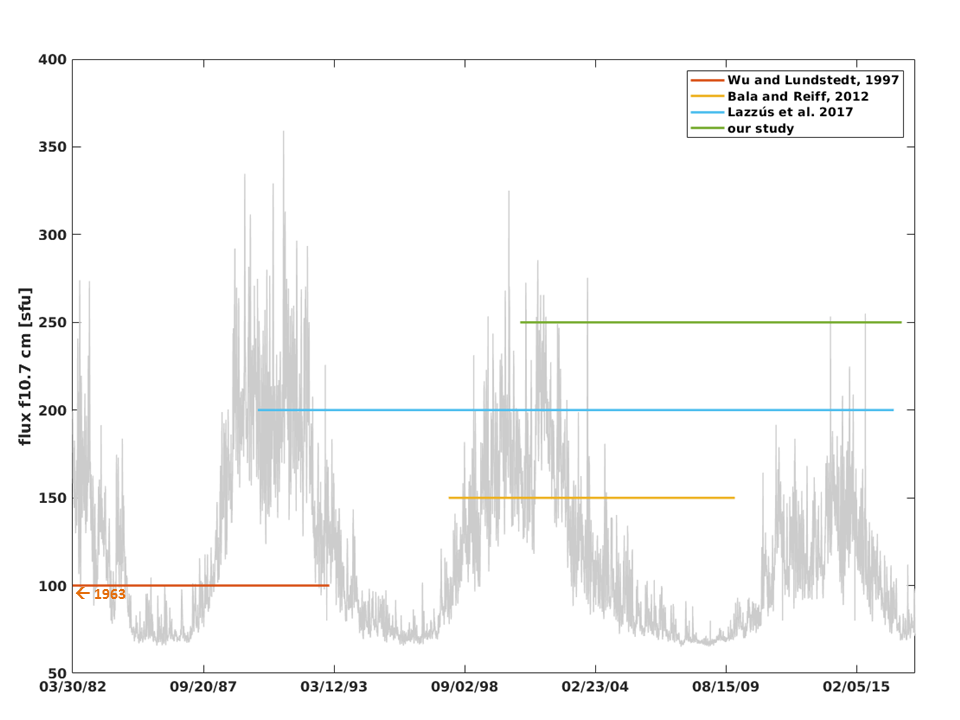
\includegraphics[width=\textwidth]{image2.png}
	\caption{Temporal coverage of database used in this study and in previous studies. \citet{wu1997geomagnetic} 
	is in orange and their database starts in 1963, \citet{Bala2012} is in yellow, \citet{Lazzus} is in blue, and our study is in green. 
	The f10.7 in grey represents the variation of solar activity.}
	\label{fig:datacoverage}
\end{figure}


The solar wind parameters and the geomagnetic Dst index are taken from the OMNI data set 
\footnote{\url{https://omniweb.gsfc.nasa.gov/ow.html}} maintained by the National Space Science 
Data Center (NSSDC) of National Aeronautics and Space Administration (NASA).

We also consider GPS data which are provided by the National Oceanic and Atmospheric Administration 
(NOAA). This dataset was provided by the team working on the Combined X-ray dosimeter or CXD at the 
Los Alamos National Laboratory 
\footnote{\url{https://www.ngdc.noaa.gov/stp/space-weather/satellite-data/satellite-system/gps/}}. 
In this study, we decided to use data recorded by the GPS satellite ns41, which has the widest 
temporal coverage \citep{morley2017energetic}. 

\Cref{fig:datacoverage} shows the temporal coverage of the database used in this study compared 
with previous studies. The temporal coverage of our study is represented by the green line. As GPS 
ns41 data starts at $00:00$ $14$ January $2001$, we consider a set of $134,398$ hourly data points 
consisting of solar wind parameters, geomagnetic Dst index, and GPS data between this starting 
date and $23:00$ $31$ December $2016$. This includes $49$ storm events, which are listed in 
\cref{table:teststormsgpnn}. Some of these events in \cref{table:teststormsgpnn} also overlap with 
events included in \citet{Ji2012} and \citet{ChandorkarDst}. 

Studies done in the past to predict the geomagnetic index Dst have shown that various solar wind 
parameters are of interest when improving performance of Dst models. In the present study, we 
focused on the use of the solar wind density $n$, velocity $V_{\text{sw}}$, the interplanetary 
magnetic field strength $\rvert\rvert\mathbf{B}\rvert\rvert$, and its north-south component 
$B_{z}$. Concerning parameters provided by the GPS satellite ns41, we use its magnetic field
measurement, $B_{\text{gps}}$.

\section{Methodology}\label{sec:methodgpnn}

\subsection{Long Short-Term Memory Network}\label{sec:lstmintro}

The long short-term memory network (LSTM) belongs to the family of 
\emph{recurrent neural networks} (RNN). In an RNN, hidden layers are built to allow information 
persistence. They behave as a loop to allow information to be passed from one cell of the network 
to the next. When this loop is unrolled, the RNN can then be thought as multiple copies of the same 
network. The RNN architecture is particularly suited for time series forecasting applications. 

\citet{hochreiter1991untersuchungen,bengio1994learning} underlined a weakness of RNNs. They are 
supposed to connect past information to the present, but if the information needed is too far in 
the past, RNNs are unable to to retain it. This failure is due to the well known 
\emph{vanishing gradient problem} occurring during the training of RNNs. 

LSTM networks are designed to overcome the vanishing gradient problem by retaining information 
pertaining to long range temporal dependencies in time series data. LSTMs have a chain-like 
structure like RNNs, but the repeating module known as the LSTM cell has specific characteristics.

\Cref{fig:lstmcell} shows the computational graph of the LSTM cell. The two elements fundamental to 
this cell are the cell state and the gates. The cell state $\mathbf{c}_{t}$ in \cref{fig:lstmcell} 
is like a conveyor belt which is connected to various gates. Gates can add or remove information 
from the cell state depending on the information required by the LSTM unit. The important pieces of 
this architecture are: 
\begin{enumerate*} 
	\item the forget gate $\mathbf{f}_t$,
	\item the input gate $\mathbf{i}_t$, 
	\item the cell state $\mathbf{c}_t$, and
	\item the output gate $\mathbf{o}_t$  
\end{enumerate*}  

\begin{figure}
	\noindent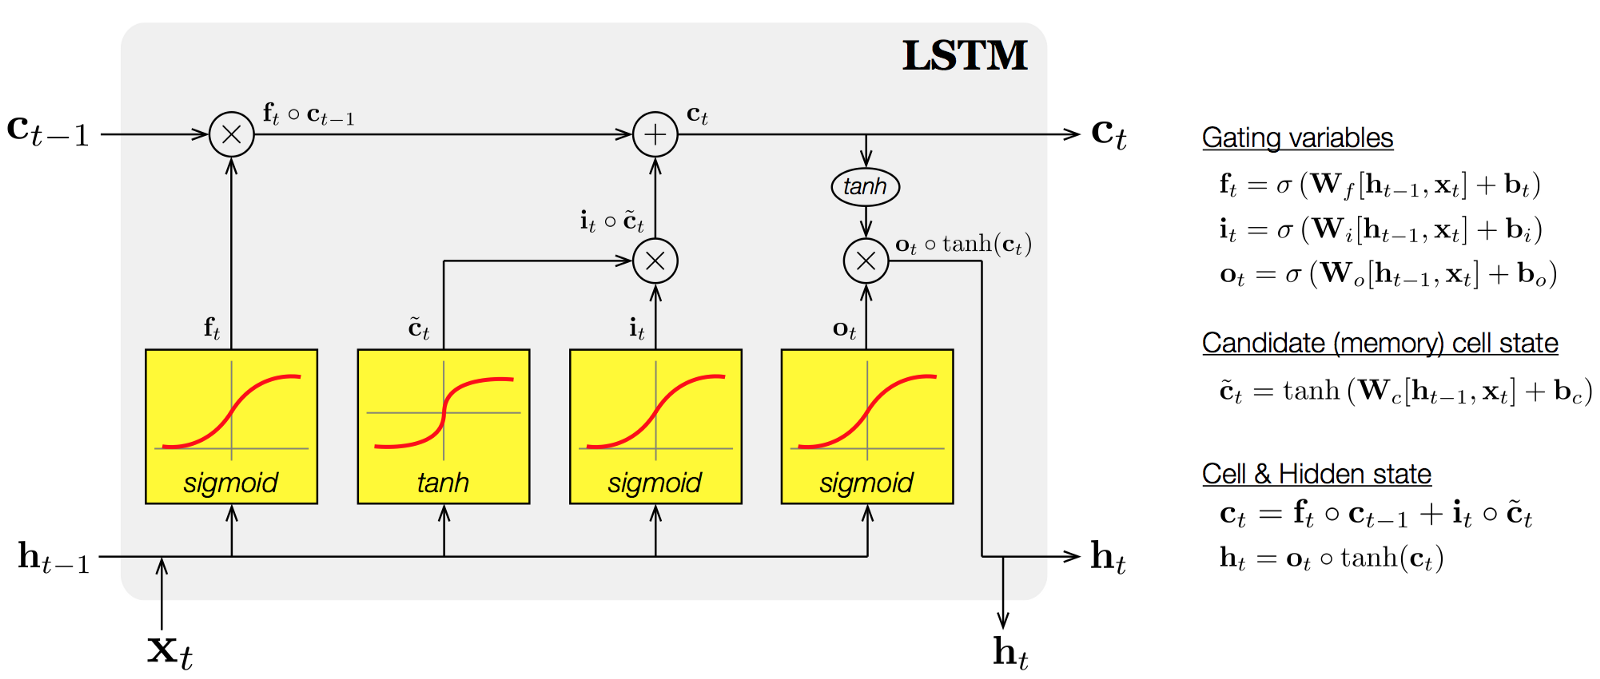
\includegraphics[width=\textwidth]{lstm.png}
	\caption{Schematic diagram of the LSTM cell. Reproduced 
	from \url{https://github.com/llSourcell/LSTM_Networks/blob/master/LSTM\%20Demo.ipynb}}
	\label{fig:lstmcell}
\end{figure}

\subsubsection*{Forget Gate \& Input Gate}

The forget gate is expressed as 
%
\begin{equation}\label{eq:forgetgate}
 \mathbf{f}_{t} = \sigma  \left( \mathbf{W}_f \boldsymbol{\cdot}  \left[ \mathbf{h}_{t-1}, \mathbf{x}_t \right] + 
 \mathbf{b}_f \right) \ ,
\end{equation}
%
where $\sigma$ is the component wise sigmoid function and  $\mathbf{W}_{f}$ and $\mathbf{b}_{f}$ 
are the weight matrix and bias vector of the gate respectively. This notation is kept for 
subsequent equations. The forget gate compares the information coming from the previous cell 
$\mathbf{h}_{t-1}$ and the incoming information $\mathbf{x}_{t}$, and outputs a number between 
zero and one. Zero is achieved if the information is entirely discarded, and one is given if it 
is altogether retained.
%
Correspondingly, the input gate in \cref{eq:inputgate} decides what information is retained, depending 
on past hidden cell state $\mathbf{h}_{t-1}$ and exogenous inputs $\mathbf{x}_t$. $\mathbf{W}_{i} $ and  
$\mathbf{b}_{i}$ are the weight matrix and bias vector of the input gate respectively.
%
\begin{equation}\label{eq:inputgate}
 \mathbf{i}_{t} = \sigma  \left(\mathbf{W}_{i} \boldsymbol{\cdot} \left[ \mathbf{h}_{t-1}, \mathbf{x}_{t} \right] + 
 \mathbf{b}_{i} \right)
\end{equation}

\subsubsection*{Cell State}

The inputs $\mathbf{x}_t$ and cell hidden state $\mathbf{h}_{t-1}$ are then passed through a 
hyperbolic tangent transformation to create a vector of candidate values $\tilde{\mathbf{c}}_{t}$ 
as per \cref{eq:candidate}. This candidate state $\tilde{\mathbf{c}}_{t}$ is used to create the 
updated cell state $\mathbf{c}_{t}$, $\mathbf{W}_{c}$  and  $\mathbf{b}_{c}$ being the weight and 
bias of this layer respectively.
%
\begin{equation}\label{eq:candidate}
 \tilde{\mathbf{c}}_{t} = \text{tanh} \left( \mathbf{W}_{c} \boldsymbol{\cdot}  \left[ \mathbf{h}_{t-1},\mathbf{x}_t \right] + 
 \mathbf{b}_{c} \right)
\end{equation}
%
The new cell state $\mathbf{c}_t$ is computed as a weighted sum of the old cell state 
$\mathbf{c}_{t-1}$ and the candidate cell state $\tilde{\mathbf{c}}_{t}$. This is expressed as 
%
\begin{equation}\label{eq:newstate}
 \mathbf{c}_t = \mathbf{f}_{t} \circ \mathbf{c}_{t-1} + \mathbf{i}_{t} \circ \tilde{\mathbf{c}}_{t} \ ,
\end{equation}
where $\circ$ denotes the element wise (Hadamard) product. The old cell state is appropriately 
\enquote{forgotten} using the output of $\mathbf{f}_t$, and information from the candidate state 
is allowed to enter $\mathbf{c}_t$ using $\mathbf{i}_t$.

\subsubsection*{Output Gate \& Prediction}

The output of the LSTM cell is calculated using \cref{eq:outputgate}. First, the sigmoid 
transformation helps to define the output $\mathbf{o}_t$. Second, the hidden state $\mathbf{h}_t$ 
is computed by multiplying $\mathbf{o}_{t}$ with a hyperbolic tangent transformation of the cell 
state $\mathbf{c}_{t}$. The value of $\mathbf{h}_{t}$ (seen in \cref{fig:lstmcell}) becomes the 
final prediction computed LSTM cell for input $\mathbf{x}_t$.
%
\begin{align} \label{eq:outputgate}
	\mathbf{o}_{t} &= \sigma \left( 
		\mathbf{W}_o \boldsymbol{\cdot} \left[\mathbf{h}_{t-1}, \mathbf{x}_{t} \right] + \mathbf{b}_o \right) \\
	\mathbf{h}_{t} &= \mathbf{o}_{t} \circ \text{tanh}(\mathbf{c}_t)
\end{align}

\subsection{The LSTM Dst Model}\label{sec:lstmDstArch}

To produce predictions of Dst up to six hours ahead, we trained six LSTM models. Thus for every 
input, we obtained a vector of outputs 
$[\mathrm{\hat{D}st}\left(t + p\right)], p\in \{ 1, \cdots, 6 \}$.
%
For inputs $\mathbf{x}_t$, we use solar wind parameters 
($n$, $V_{\text{sw}}$, $|\mathbf{B}|$, $B_{z}$) and the GPS data ($B_{\text{gps}}$) described in 
\cref{sec:datagpnn}. We also use the time history of Dst, from one to six hours back.
%
\begin{equation}\label{eq:lstminputs}
	\begin{aligned}
		\mathbf{x}_t &= (n \left( t \right) , V_{\text{sw}}\left( t \right), 
		|\mathbf{B}\left( t \right)|, B_{z}\left( t \right) , B_{\text{gps}} \left( t \right),\\ 
		& \ \  \ \  \ \mathrm{Dst} \left( t-1 \right), \mathrm{Dst} \left( t-2 \right) , \ldots , 
		\mathrm{Dst} \left( t-6 \right) )
	\end{aligned}
\end{equation}

\subsubsection*{Architecture \& Implementation}

LSTM cells can be \emph{stacked} such that the output of one cell provides the input for the next. 
One may construct LSTM stacks of increasing size depending on the task at hand.  

In \cref{eq:dstmodel,eq:lstmstack}, we describe the Dst prediction architecture. The $p$ hour 
ahead prediction $\mathrm{\hat{D}st} \left(t + p \right)$ is the output of the function 
$m^{p}_{\text{NN}}(\cdot)$, which is obtained by successive operation of $d$ LSTM cells. 
Mathematically this is equivalent to function composition 
$h^{p}_{d} ( h^{p}_{d-1}( \cdots (h^{p}_{1}(\cdot)\cdots))$.
%
\begin{align}
	\mathrm{\hat{D}st} \left(t + p \right) &= 
	m^{p}_{\text{NN}} (\mathbf{x}_t) \label{eq:dstmodel}\\
	m^{p}_{\text{NN}} (\mathbf{x}_t) &= 
	h^{p}_{d} ( h^{p}_{d-1}( \cdots (h^{p}_{1}(\mathbf{x}_t)\cdots)) \label{eq:lstmstack}
\end{align}

To find the LSTM structure, which is most suitable for predicting geomagnetic activity, we 
built networks consisting of varying number of cells. After training and validating each candidate 
architecture, the best performing LSTM network was chosen as the mean function for the Gaussian 
process component outlined in \cref{sec:gpcomponent}.

The LSTM component of the GPNN model was implemented using the Lasagne library in Python 
\citep{lasagne,theanoshort}. 

\subsection{LSTM Model Training}

The LSTM architecture can be trained with an iterative backpropagation based optimization 
algorithm. Unlike the case of RNN network training, the vanishing gradient problem does not 
persist. A number of stochastic gradient based variants are used for training neural networks, 
such as, but not limited to, \emph{Levenburg - Maquardt} \citep{marquardt1963algorithm}, 
\emph{Nesterov Accelerated Gradient} (NAG) \citep{nesterov1983method}, adaptive learning rates 
for each network weight \citep{SilvaAlmeida}, adaptive gradient based methods such as AdaGrad 
\citep{duchi2011adaptive}, and adaptive learning rate methods like RMSprop 
\citep{tieleman2012lecture}. 

In this work, we use the RMSProp algorithm for training the LSTM component of the GPNN model. 
Below we give a brief explanation of its functioning.

\subsubsection*{The RMSProp Algorithm}

For the purposes of notational simplicity, the weights and biases of the LSTM architecture are 
concatenated into a single vector $\mathbf{\theta}$, where $\theta_i$ denotes an individual 
scalar element of $\mathbf{\theta}$ and $\theta^{k}_{i}$ the value of $\theta_i$ at iteration $k$. 
The quantity $J(\mathbf{\theta})$ is the objective function which defines how well the outputs of 
the LSTM model fit the observed data. The training process of the LSTM consists of computing an 
approximate minimum of $J(\mathbf{\theta})$. We define $g_{k,i}$ in \cref{eq:gradient} as the 
gradient of the objective function with respect to the parameter $\theta_{i}$ at iteration $k$. 
%
\begin{equation}\label{eq:gradient}
 g_{k,i} = \left. \frac{\partial{J}(\mathbf{\theta})}{{\partial \mathbf{\theta}_i}}\right\rvert_{\theta = \theta^k}
\end{equation}
%
The aim of the training process is to successively decrease the value of $J(\mathbf{\theta})$ over 
a number of training iterations. This is achieved as follows.

First, the running average of the second order moment of the gradients 
$\mathrm{E} \left( g^{2} \right)$ is computed at each iteration $k$. Then, the updated parameters 
$\theta^{k+1}_{i}$ are calculated using the gradient $g_{k,i}$ and a damped learning rate of 
$\frac{\eta}{\sqrt{\mathrm{E} \left[ g^{2} \right]_{k,i}} + \epsilon }$ ($\epsilon$ is a small 
number added to $\sqrt{\mathrm{E} \left[ g^{2} \right]_{k,i}}$ to prevent numerical overflow). The 
update of parameters using RMSprop can then be computed using \cref{eq:learningrmsprop}.
%
\begin{align}\label{eq:learningrmsprop}
 \mathrm{E} \left[ g^{2} \right]_{k+1,i} &= 0.9 \mathrm{E} \left[ g^{2} \right]_{k,i} + 0.1 g_{k,i}^{2}  \\ 
 \theta^{k+1}_{i} &= \theta^{k}_{i} - \frac{ \eta }{\sqrt[]{\mathrm{E} \left[ g^{2} \right]_{k,i}} + \epsilon } g_{k,i}
\end{align}

\subsection{Gaussian Processes}\label{sec:gpcomponent}

Gaussian processes are a family of models that provide a principled probabilistic framework for 
forecasting. GP models output a predictive distribution instead of a point forecast. Starting from 
a \emph{prior distribution}, GP models construct a \emph{posterior predictive distribution}. The 
appeal of using GP models is that, their practical implementation is straightforward boiling down 
to a simple analytical expression that requires no more than linear algebra, although their 
theoretical formulation is general. In this study, the GP component is implemented using the GPML 
Matlab software package \citep{rasmussen2010gaussian}. 

We will not give a complete review of the GP methodology here. The interested reader can refer to 
\cref{sec:osaGPmethod} for a detailed review of Gaussian process models and their 
mathematical formulation.

A GP is completely specified by its mean function  $m \left( \mathbf{x} \right)$ and its covariance 
function or \emph{kernel} $K (\mathbf{x}, \mathbf{x}')$ in \cref{eq:gpformulation}.

\subsubsection*{Kernel Function}

Kernels determine how each point $\mathbf{x}_t$ influences the values that the GP will have on 
another point $\mathbf{x}_s$. The main idea is that if $K(\mathbf{x}_t, \mathbf{x}_s) \gg 0$, we 
expect the output from the GP model at these points to be statistically correlated. 
%
\begin{equation}\label{eq:gpcov}
	K_{\text{NN}} \left( \mathbf{x}, \mathbf{x}' \right) = 
	\frac{2}{ \pi } \text{sin}^{-1} \left( \frac{2\mathbf{x}\boldsymbol{\cdot}\mathbf{x}'}{
		\sqrt{ \left( 1+2\mathbf{x}\boldsymbol{\cdot} \mathbf{x} \right)}\sqrt{\left( 1+2\mathbf{x}'\boldsymbol{\cdot}\mathbf{x}' \right)}
		} \right)
\end{equation}


Kernels often introduce assumptions about the continuity of the functions that will be 
represented by the resulting GP regression model. \citet[ch.~4]{Rasmussen:2005:GPM:1162254} gives an 
introduction to common kernels used in machine learning applications and the type of continuity assumptions 
of their resulting GP models. In this study, we use the neural network kernel \citep{williams1998computation} 
described in \cref{eq:gpcov}. 

\subsubsection*{Mean Function}

The mean function $m \left( \mathbf{x} \right)$ defines an a priori mean value of the GP predictive distribution for 
some input $\mathbf{x}$. It is quite common to set $m(\mathbf{x}) = 0$ without loss of generality for situations where 
it is difficult to define an a priori expression for the predictive mean. 
\citet[ch.~2,sec.~2.7]{Rasmussen:2005:GPM:1162254} states that using mean functions is a good way to incorporate 
domain knowledge or to augment the model's capabilities in capturing complex behavior. This outlines the structure 
of the hybrid GPNN model consisting of an LSTM and GP components. 

\subsection{The GPNN Model}

\begin{align}
	\mathrm{Dst} \left( t+p \right) &= f_{p} \left( \mathbf{x}_{t} \right) + \epsilon \label{eq:dstgpnn}\\ 
	\epsilon &\sim N \left( 0, \sigma ^{2} \right)  \label{eq:gpnnNoise}\\
	f_{p} \left( \mathbf{x}_{t} \right)  &\sim 
	\mathcal{GP}\left(m^{p}_{\text{NN}}(\mathbf{x}_t), K_{NN}(\mathbf{x}_{t},\mathbf{x}_{s})\right)\label{eq:gpnnGPForm}
\end{align}
	
In \cref{eq:dstgpnn,eq:gpnnNoise,eq:gpnnGPForm}, we give a formal specification of the proposed GPNN model in 
terms of the notations introduced in \cref{sec:osaGPmethod}. The ground truth $\mathrm{Dst}\left(t + p\right)$ 
is assumed to be the result of a Gaussian Process $f_{p}$ corrupted by Gaussian measurement noise $\epsilon$, 
with $p = {1,2,3,4,5,6}$ being the forecast horizon going from one to six hours ahead. The mean function of the 
Gaussian process $f_{p}$ is set to $m^{p}_{\text{NN}} \left( \mathbf{x} \right)$ described in 
\cref{sec:lstmDstArch} and the covariance is set to the neural network covariance function 
from \cref{eq:gpcov}. 


\section{Experiments} \label{sec:resultsgpnn}

\begin{figure}
	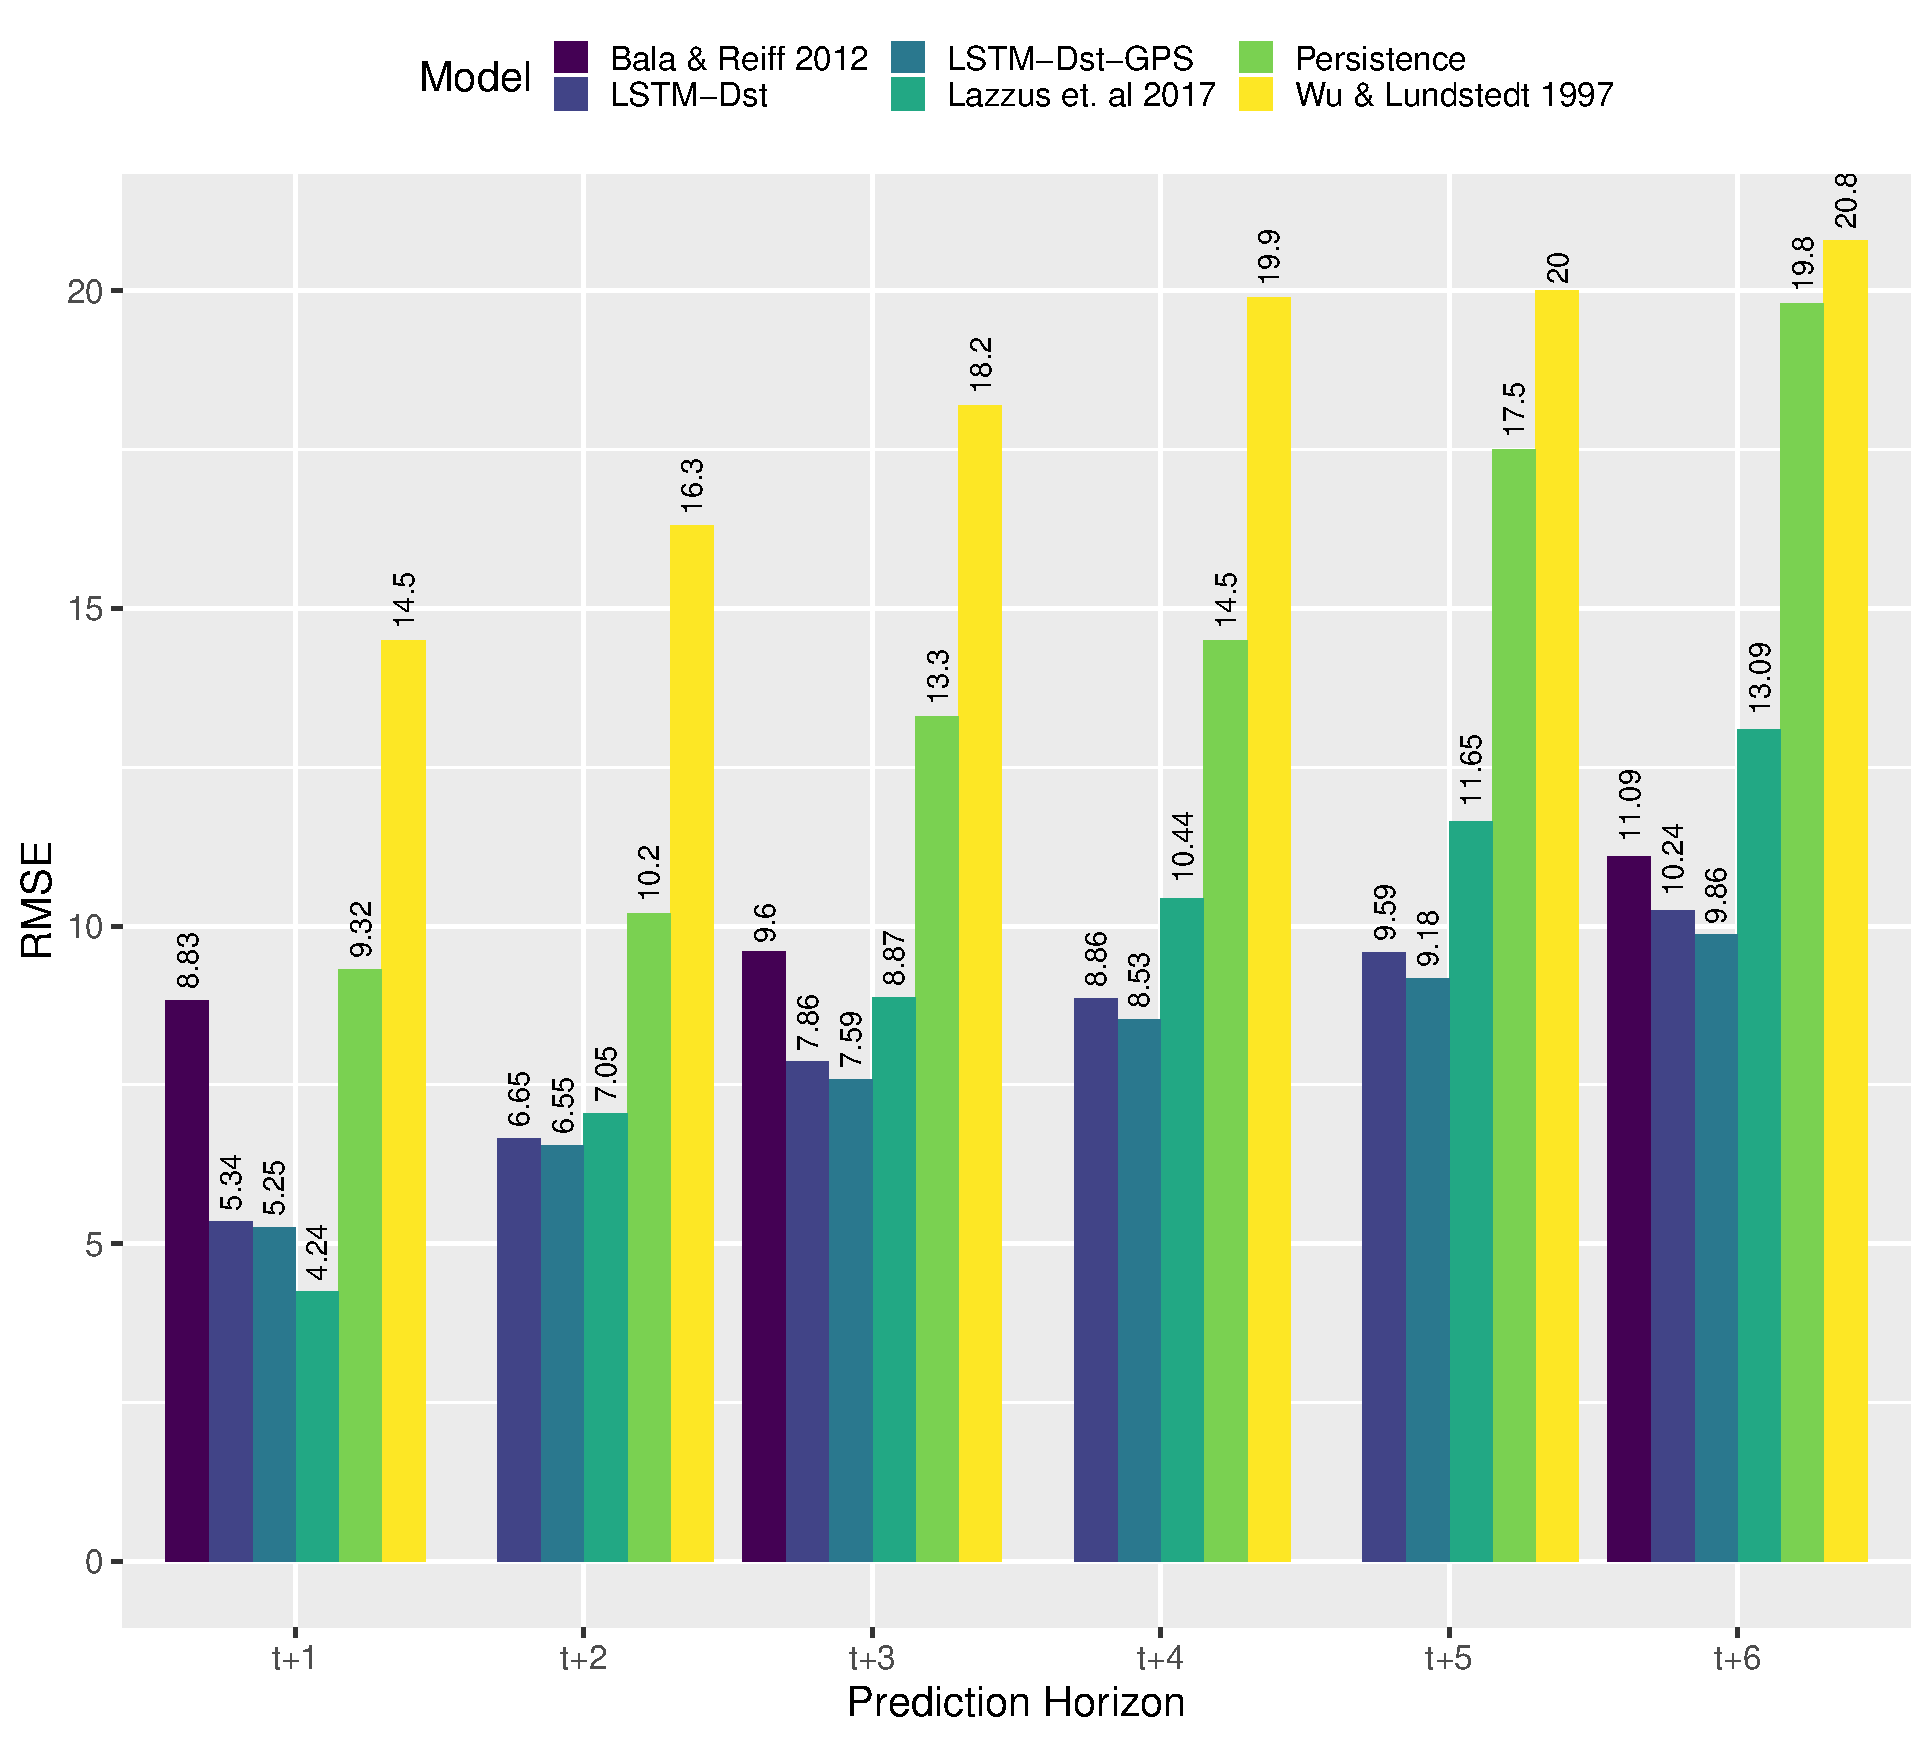
\includegraphics[width=\textwidth]{lstmCompRMSE.pdf}
	\caption{$\mathrm{RMSE}$ comparison of $\mathrm{Dst}$ forecast models.}
	\label{fig:lstmRMSE}
\end{figure}

\begin{figure}
	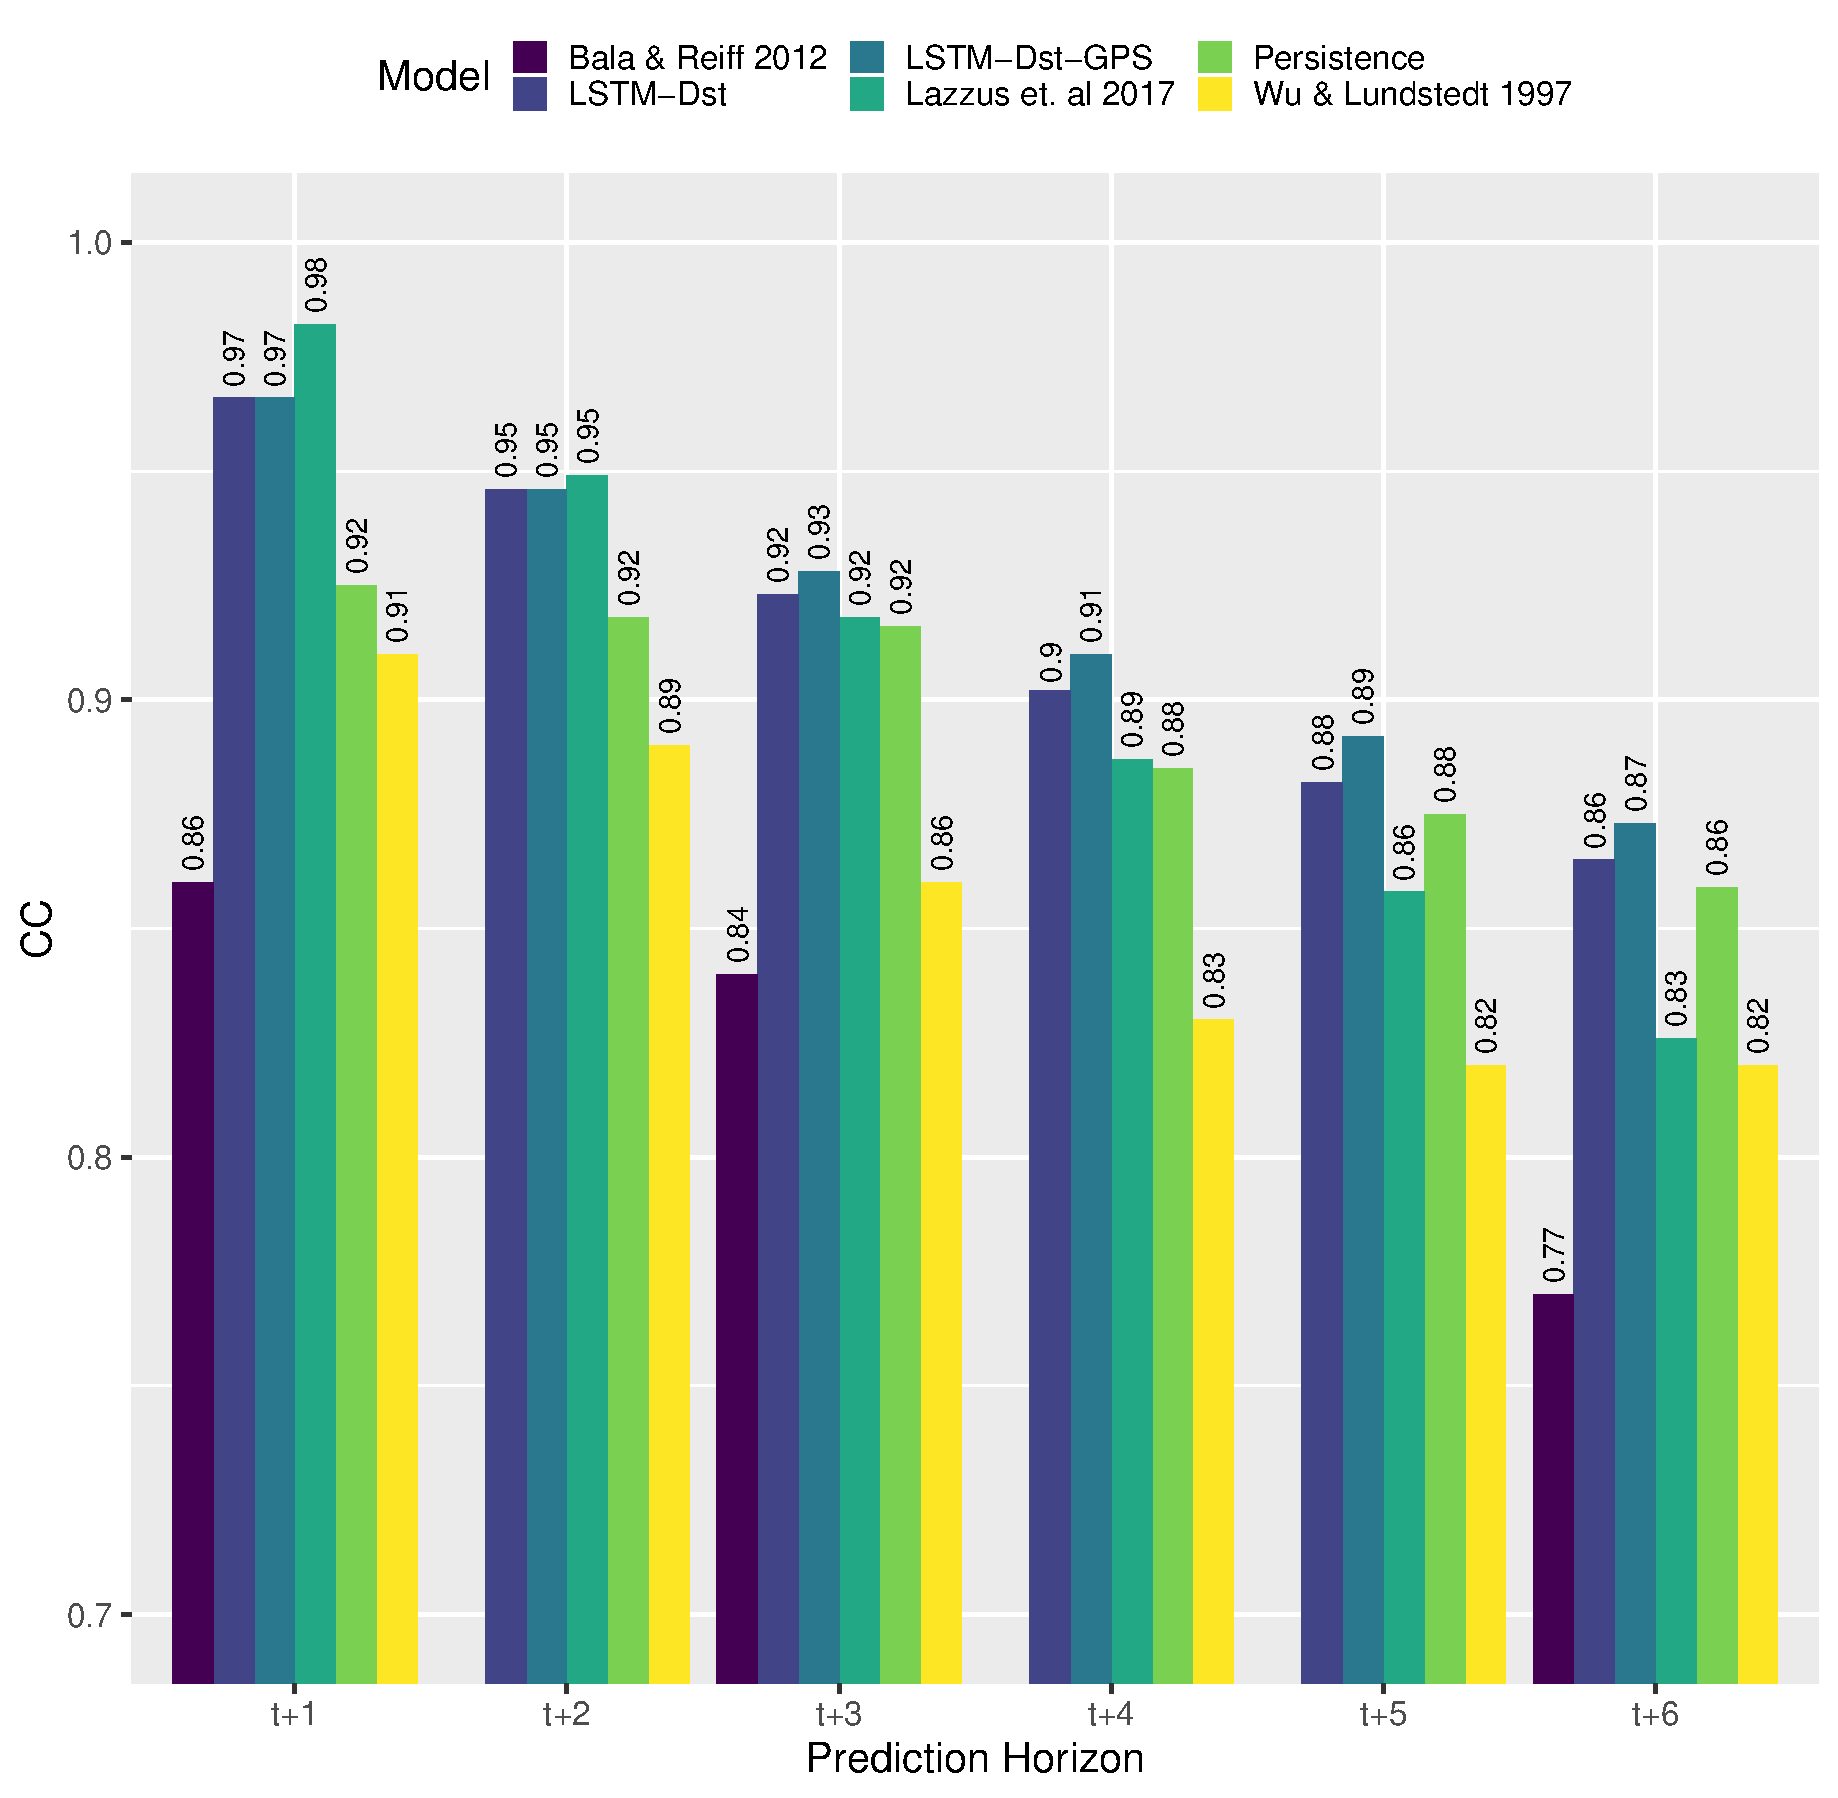
\includegraphics[width=\textwidth]{lstmCompCC.pdf}
	\caption{$\mathrm{CC}$ comparison of $\mathrm{Dst}$ forecast models.}
	\label{fig:lstmCC}
\end{figure}

\subsection{LSTM Model Evaluation}

For the purposes of training and evaluation, the data set is divided as follows: $70\%$ for 
training, $20\%$ for testing and $10\%$ for validation. The LSTM model is evaluated using the 
root mean square error (RMSE) and the Pearson correlation coefficient (CC) defined by 
\cref{eq:rmse,eq:cc} respectively. Based on the performance calculated on the validation data, an 
LSTM network of depth $d = 20$ cells was chosen as the mean function of the GPNN model.
%
\begin{equation}\label{eq:rmse}
 \mathrm{RMSE} = \sqrt[]{\sum_{t=1}^{n}\left( 
	 \mathrm{Dst} \left( t \right) - \mathrm{\hat{D}st}\left(t\right)
 \right) ^{2}/n}
\end{equation}
%
\begin{equation}\label{eq:cc}
 \mathrm{CC} = \frac{\Cov(
	 \mathrm{Dst},\mathrm{\hat{D}st})}{
		 \sqrt[]{
			 \Var(\mathrm{Dst}) \Var(\mathrm{\hat{D}st})
		 }
	} 
\end{equation}
%
In order to give context for the performance of our LSTM model, we compare the following models for Dst predictions 
for the time horizon $t+1 \cdots t+6$, summarised in \cref{table:competingmodels}.

\begin{table}[ht]
	\centering
	\caption{Summary of Dst forecasting models compared in this study}
	\label{table:competingmodels}
	\begin{tabular}{ l  p{0.65\textwidth} }
		\hline
		\textbf{Model} & \textbf{Description}\\
		\hline
		\citet{wu1997geomagnetic} & An Elman RNN model having explicitly computed solar wind magnetospheric 
		coupling functions as inputs.\\
		\citet{Bala2012} & A feedforward neural network model using the \emph{Boyle} function as input.\\
		\citet{Lazzus} & A feedforward neural network model using only the time history of Dst. Trained using 
		particle swarm optimization.\\
		Persistence model & $\mathrm{\hat{D}st}(t + p) = \mathrm{Dst}(t)$, also used for benchmarking in 
		\cref{sec:gpOSAEval}.\\
		LSTM-Dst & Our proposed LSTM model. Inputs are solar wind parameters (\cref{sec:datagpnn}) 
		and time history of Dst.\\
		LSTM-Dst-GPS & The LSTM model but with GPS magnetic field data $B_{\text{gps}}$ also included in the inputs. \\
		\hline
	\end{tabular}
\end{table}

\Cref{fig:lstmCC,fig:lstmCC} present a comparison of $\mathrm{CC}$ and $\mathrm{RMSE}$ performance 
of the $\mathrm{Dst}$ prediction models listed in \cref{table:competingmodels}. 

Our models LSTM-Dst \& LSTM-Dst-GPS provide performance which is competitive to that obtained by 
\citet{Lazzus} for one to three hours ahead. When the forecast horizon goes from four to six hours 
ahead, LSTM-Dst \& LSTM-Dst-GPS provide better global performance. As an example, when considering 
a six-hour-ahead forecast, LSTM-Dst-GPS provides a CC of $0.873$ and a RMSE of 
$\SI{9.86}{\nano\tesla}$, while \citet{Lazzus} obtained a CC of $0.826$ and a RMSE of 
$\SI{13.09}{\nano\tesla}$. The model presented in \citet{Lazzus} uses only time history of Dst. 
This emphasises the performance benefits of using exogenous data when predicting geomagnetic 
activity with a time horizon greater than one hour. 

\citet{Bala2012} used the Boyle index as an input function and obtained competitive RMSE 
performance to LSTM for six hour ahead predictions. Their model presents a\ CC of $0.77$ and a 
RMSE of $\SI{11.09}{\nano\tesla}$.
%
\begin{figure}
	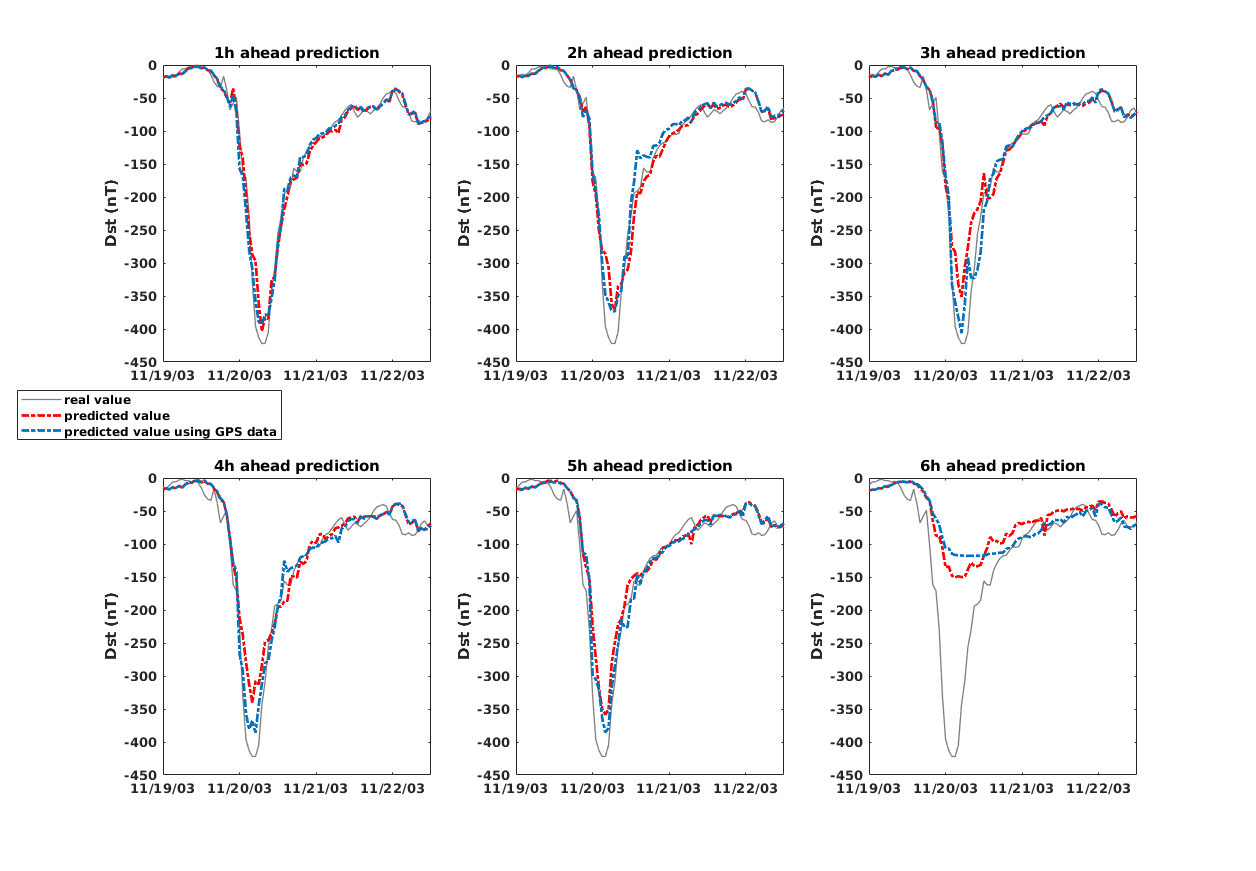
\includegraphics[width=\textwidth]{image5.png}
	\caption{$\mathrm{Dst}$ predictions made by the LSTM-Dst and LSTM-Dst-GPS models for the 2003 Halloween storm.}
    \label{fig:lstmhalloween}
\end{figure}
%
The Elman RNN proposed in \citet{wu1997geomagnetic} is an important benchmark for the GPNN model 
because the LSTM architecture is a more sophisticated form of the RNN structure. 
\citet{wu1997geomagnetic} provided for a six ahead forecast, a CC of $0.82$ and a RMSE of 
$\SI{20.8}{\nano\tesla}$. The LSTM architecture thus offers performance benefits over standard 
RNNs when making geomagnetic activity.
 
We observed that using GPS data generally results in an improved forecasts of important geomagnetic 
storm events. \Cref{fig:lstmhalloween} presents forecasts produced the LSTM-Dst in blue and 
LSTM-Dst-GPS in red for the $2003$ Halloween storm event 
(maximum strength of $\SI{-422}{\nano\tesla}$). Predictions for one to two hours ahead are very 
similar, but when we consider the forecasts made for three hours ahead, LSTM-Dst predicts a storm 
peak of $\SI{-348}{\nano\tesla}$ while LSTM-Dst-GPS provides a prediction of 
$\SI{-405}{\nano\tesla}$. 

For a four-hour-ahead forecast, LSTM-Dst predicts a storm peak of $\SI{-335}{\nano\tesla}$ while 
LSTM-Dst-GPS predicts $\SI{-380}{\nano\tesla}$.



\subsection{GPNN Evaluation}

Since GP models output a predictive distribution, metrics like RMSE and CC, which are defined for 
single point predictions, are not adequate for evaluating probabilistic forecasts.

\begin{table}[ht]
	%\fontsize{8}{9.6}\selectfont
	\centering
	\caption{Storm Classification}
	\label{table:stormclass}
	\begin{tabular}{ccccc}
	\hline
	\textbf{Level of Activity} & \textbf{Storm Classification} \\ \hline
	$\mathrm{Dst} > \SI{-50}{\nano\tesla}$ & Moderate\\
	$\SI{-250}{\nano\tesla} \leq \mathrm{Dst} \leq \SI{-50}{\nano\tesla}$ & Intense\\
	$\mathrm{Dst} < \SI{-250}{\nano\tesla}$ & Super Storm\\ \hline
	\end{tabular}
\end{table}

The GPNN model provides an operator a probabilistic forecast, which can be important in a decision 
making scenario. For example, a satellite operator may choose to turn off a sensitive components or 
equipment before an intense storm, when the forecast probability of an intense event exceeds a 
predetermined trigger threshold.

Storm activity is often classified by thresholding Dst values. In line with the most common 
classification schemes, we distinguished three levels of geomagnetic activity summarised in 
\cref{table:stormclass}. It is ideal to use metrics that will be able to evaluate how well the 
GPNN model manages to correctly classify geomagnetic storms one to six hours prior. To do so, 
we used receiver operating characteristic (ROC) curves and reliability diagrams.



\subsubsection{Receiver Operating Characteristic Curve}

The ROC curve is based on a contingency table which maps how often a model correctly classifies 
outcomes when working in a binary classification setting i.e. occurrence or non occurrence of a 
predefined event, denoted by labels $1$ and $0$ respectively. From \cref{table:stormclass}, we 
constructed three binary classification problems for each storm class.

In the case of the GPNN model, we can analytically compute the probability that Dst lies within a 
particular storm class or outside it 
(e.g. $\mathbb{P}[\SI{-250}{\nano\tesla} \leq \mathrm{Dst} \leq \SI{-50}{\nano\tesla}]$ is the 
probability of occurrence of an intense storm). For any storm class, by choosing a threshold 
probability, we can assign a classification of $1$ (belonging to that storm class) if the 
probability predicted by the GPNN model is greater than the chosen threshold, and $0$ if otherwise. 

The ROC contingency table is then constructed by tabulating the relationship between the 
\emph{true positive ratio} (TPR) and \emph{false positive ratio} for varying threshold 
probabilities. A \emph{true positive} is when an occurrence of the event in question is correctly 
classified by the model as such. A \emph{false positive} is when a non-occurrence is classified as 
an occurrence. The TPR is then the ratio of true positives to the total number of event 
occurrences, while the FPR is the ratio of false positives to the number of non occurrences. 
For perfect classification, $\mathrm{FPR} = 0$ and $\mathrm{TPR} = 1$. Thus, the value of the 
threshold that produces the point closest to these values is optimal.  

In \cref{table:rocgpnn1h,table:rocgpnn2h,table:rocgpnn3h,table:rocgpnn4h,table:rocgpnn5h,table:rocgpnn6h}, 
we present ROC curves obtained from one to six hour ahead forecasts, organised by storm category. 
The ROC is usually shown graphically, but numerical values are more relevant for the reader to 
analyse variations depending on the chosen threshold probability. The optimal TPR and FPR values 
are in bold, obtained by minimising the Euclidean distance from $\text{FPR} = 0$ and 
$\text{TPR} = 1$.

For predictions done from one to five hours ahead, TPR values are always greater than $0.719$ for 
thresholds from $10\%$  to $40\%$, and then decrease with increasing thresholds. If we focus on the 
six-hour-ahead forecast, the best TPR is $0.5$ for a $10\%$ threshold. It means that the more there 
is an increasing probability for a superstorm to occur, the less the model is able to forecast it 
without misjudgments six hours in advance. However, for intense storms 
($\SI{-250}{\nano\tesla} < \mathrm{Dst} < \SI{-50}{\nano\tesla}$), the GPNN has a TPR higher 
than $0.670$ for thresholds between $10\%$ and $80\%$, and for moderate storms, this model has 
a TPR higher than $0.649$ for all thresholds, for predictions going from one to six hours ahead. 


\subsubsection{Reliability diagram}


The ROC tables discussed in the previous section give information about the ability of the 
forecasting system to detect the occurrence of geomagnetic storm events based on a chosen decision 
threshold, in terms of false and true positives. Reliability diagrams measure how closely the 
forecast probabilities of an event correspond to the actual frequency with which an event is 
observed. A perfectly reliable forecast is one in which an event predicted with probability $p$ is 
observed, on average, with frequency $p$. The reliability diagram bins the forecasts into groups 
according to the predicted probability, which is shown on the horizontal axis. The frequency with 
which an event was observed to occur for each bin is then plotted on the vertical axis. If the 
reliability curve lies above/below than the perfect diagonal slope, the resulting forecasts are 
under/over confident 
(i.e. they yield  smaller/higher probabilities for a specific outcome than observed). 

\Cref{fig:gpnnreliability} presents reliability diagrams obtained from one to six-hour-ahead 
forecasts made by the GPNN. It shows that the one-hour-ahead forecast slightly underestimates the 
likelihood of storm events when their occurrence probability is $35\%$. For example, when there is 
$80\%$ predicted chance of a storm, the real observed frequency of it is $90\%$. The GPNN provides 
reliable forecast for two-hour-ahead predictions, as the observed frequency of storm regarding the 
predicted probability lies almost perfectly on the diagonal. For predictions further than three 
hours ahead, GPNN tends to overestimate the probability of storms. 

If we focus on the six-hour-ahead prediction, when the GPNN model provides a predicted probability 
of $90\%$, the real frequency is $65\%$. GPNN $t+6$ model is thus overconfident. 

% Once the reliability diagram is obtained, 
% it is of interest to seek simple corrections to the forecast probabilities (re-calibration). This issue will be 
% investigated elsewhere in greater detail. Here, we just show \cref{fig:gpnnreliabilitysigma} that by multiplying 
% the standard deviation by a\ factor of 2 or 3, it it possible to improve the reliability for predicted probability 
% higher than $50\%$ (\cref{fig:gpnnreliability}). For example, if the predicted probability is $90\%$, 
% by multiplying sigma by 2, the corresponding real frequency is $72\%$ and if we multiply by 3 we get $80\%$. 
% This way, we managed to get closer to the diagonal, when the probability of events increase. Conversely, 
% a simple rescaling of the obtained standard deviation yields worse reliability for probabilities smaller 
% than $50\%$ .  


\begin{figure}
	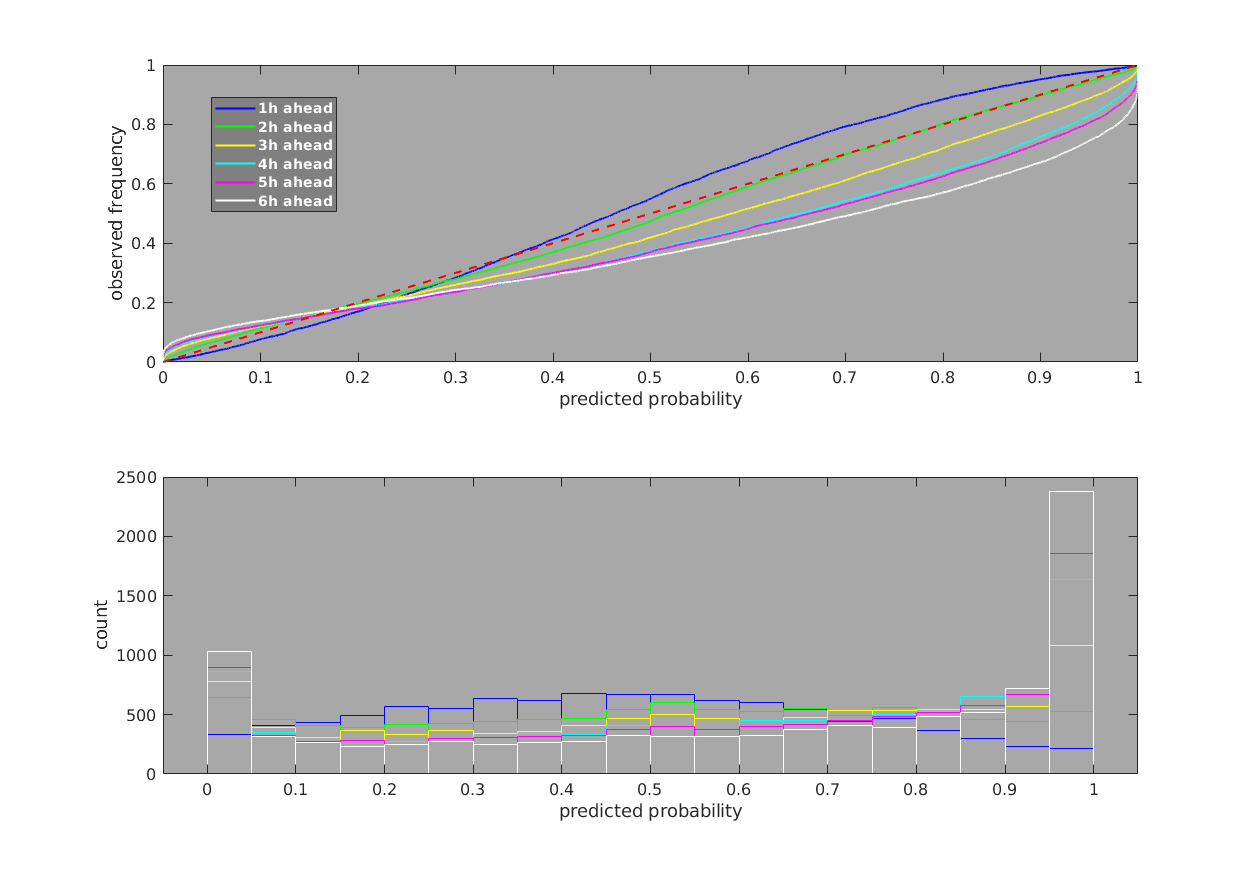
\includegraphics[width=\textwidth]{image6.png}
	\caption{Reliability diagram for Dst forecast from one to six hours ahead. The diagonal is in red dot line.}
	\label{fig:gpnnreliability}
\end{figure}


% \begin{figure}
% 	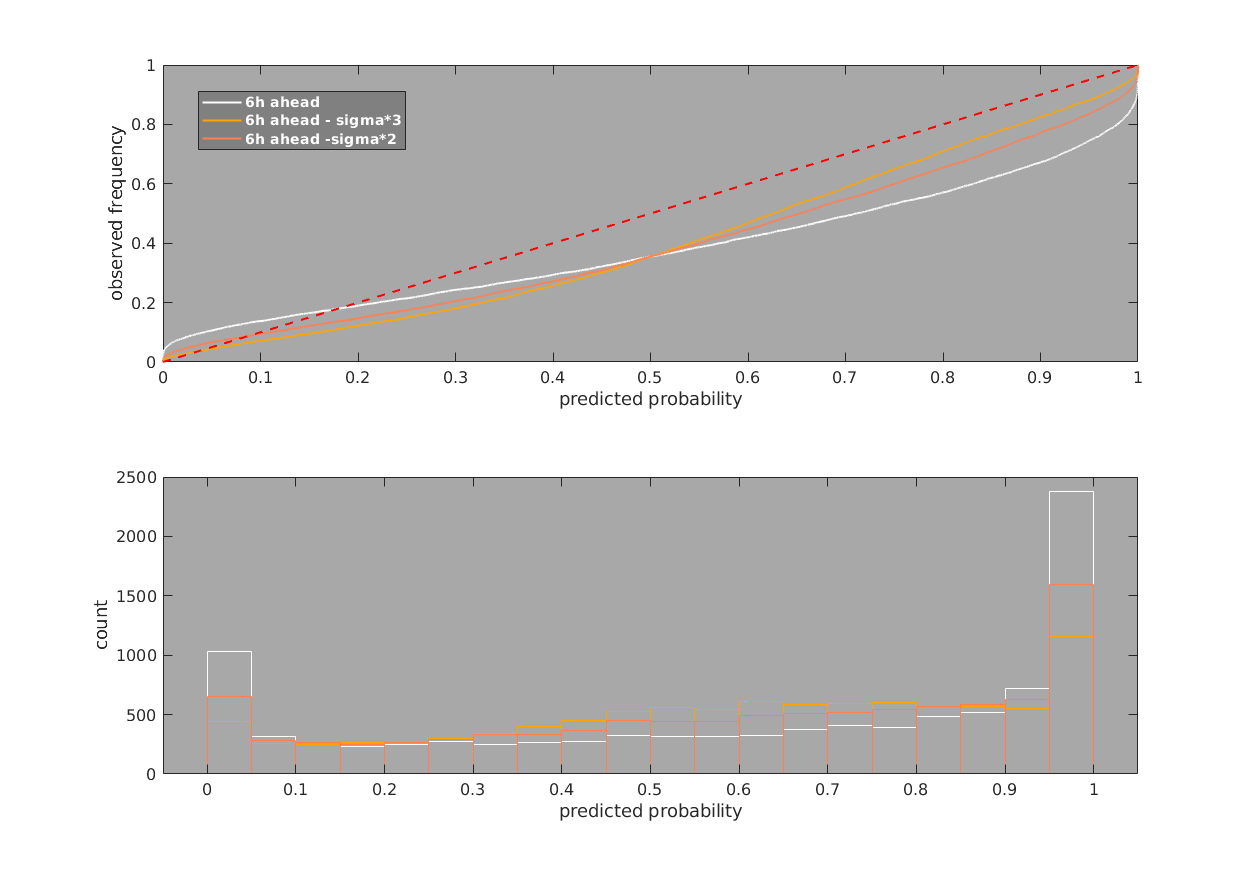
\includegraphics[width=\textwidth]{image7.png}
% 	\caption{Reliability diagram for the Dst prediction depending on the sigma value. The diagonal is in red dot line.}
% 	\label{fig:gpnnreliabilitysigma}	
% \end{figure}


\Cref{fig:gpnnhalloween} presents predictions provided by the GPNN model for the 2003 Halloween 
storm. For predictions from one to five hours ahead, GPNN provides accurate predictions with 
plausible error bars. For example, for the five hours ahead forecast, the storm peak of 
\SI{-422}{\nano\tesla} is forecasted as \SI{-391}{\nano\tesla}. 

The main benefit of the GP component in GPNN can be appreciated when comparing 
\cref{fig:lstmhalloween,fig:gpnnhalloween}, which show that the GPNN model gave more accurate 
six-hour-ahead forecasts for the $2003$ Halloween storm. The error bars calculated by the GPNN 
model include the storm peak for one to six-hour-ahead forecasts.

\begin{figure}
	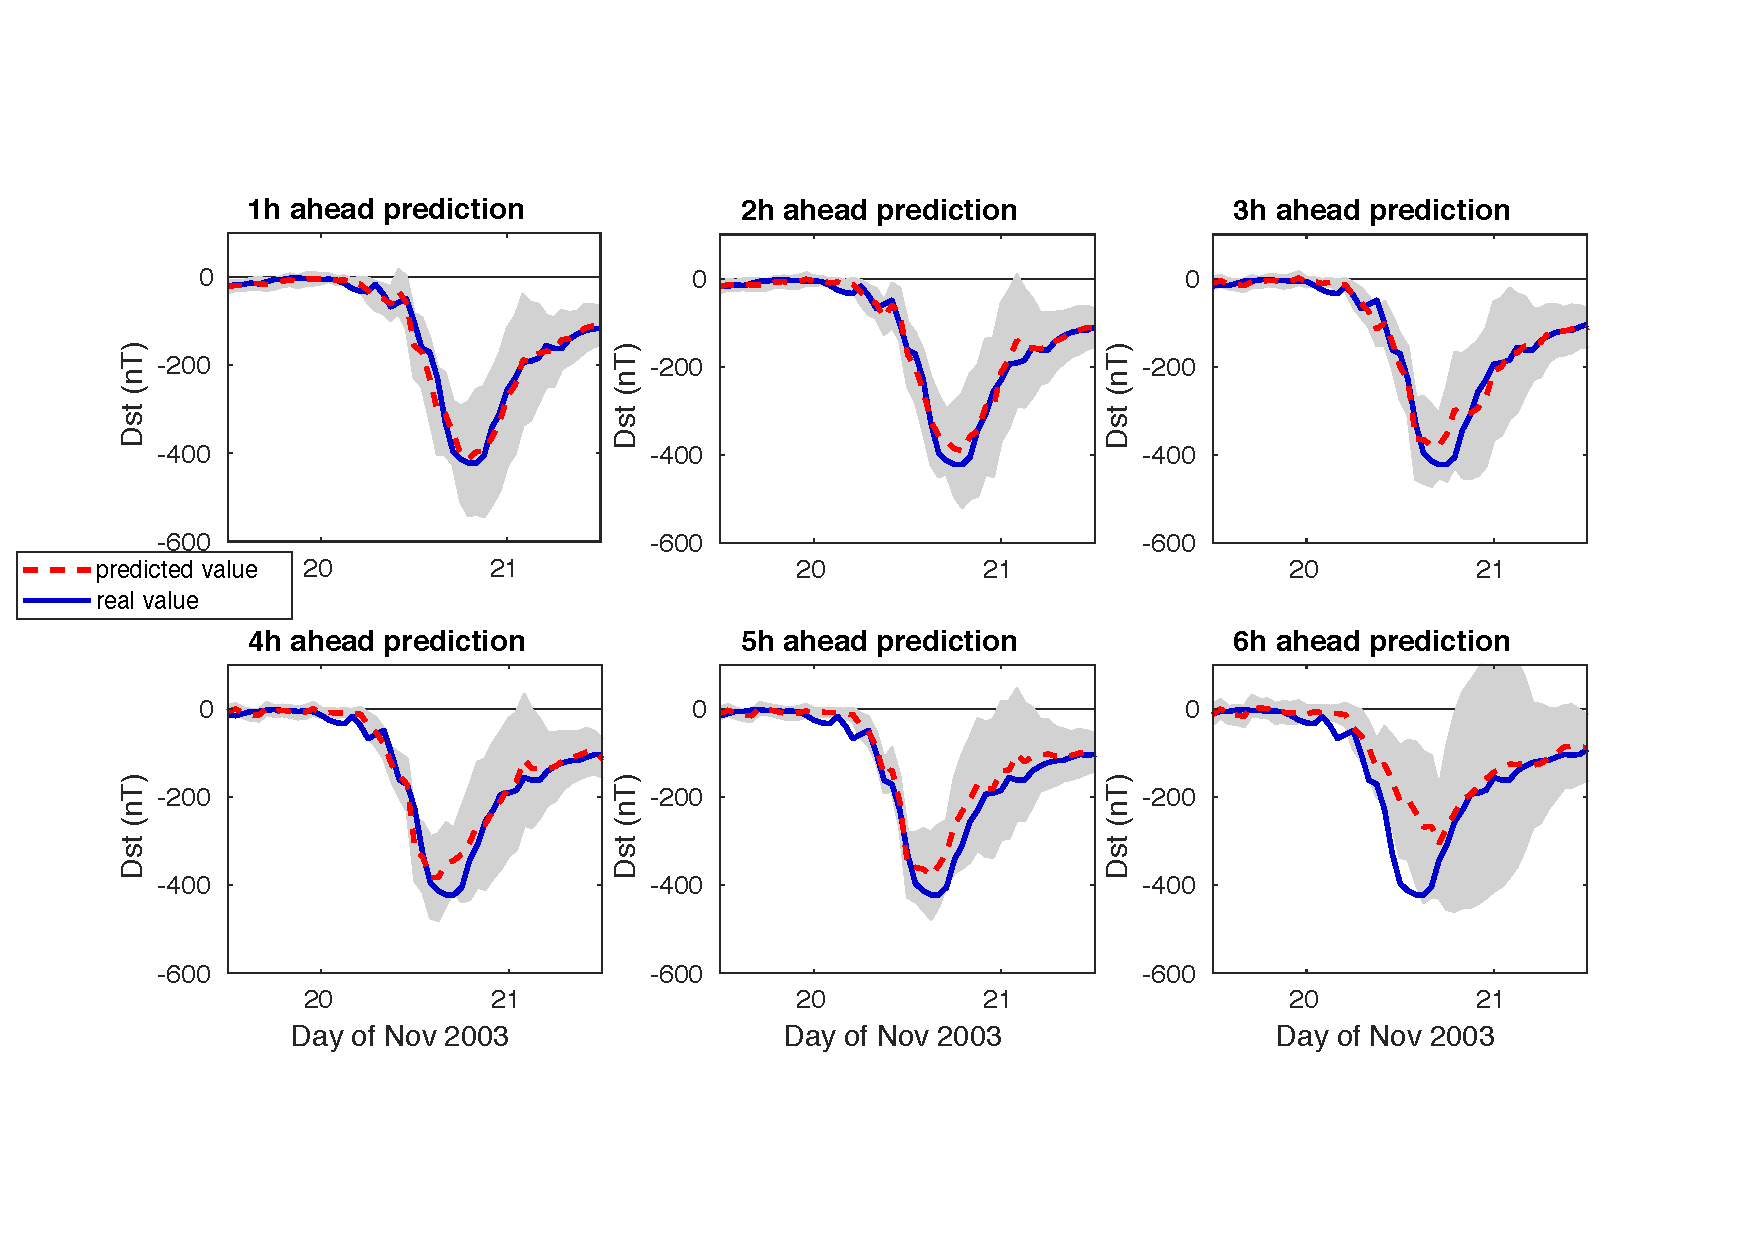
\includegraphics[width=\textwidth]{halloween_storm_GPNN.pdf}
	\caption{$\mathrm{Dst}$ predictions made by the GPNN for the 2003 Halloween storm. 
	The most probable prediction is the dotted purple line. 
	The ground truth $\mathrm{Dst}$ is the deep blue line. 
	The grey shadow represents $\pm\sigma$ error bars on the prediction.}
    \label{fig:gpnnhalloween}
\end{figure}



\section{Conclusion}


In this chapter, we presented a hybrid model for Dst forecasting, the GPNN, based on LSTM 
networks and Gaussian Processes. 

First, we developed a LSTM network to provide Dst predictions one to six hours ahead. A separate 
LSTM was developed for each time step of the forecast horizon, then the global performance of LSTM 
was compared to previously proposed neural network based Dst forecast models. We observed that the 
LSTM provides competitive performance in comparison to the state of the art in Dst forecasting. 
When focusing on extreme events like the well known $2003$ Halloween storm, we noted that even 
though our model's global performance metrics are excellent, the six-hour-ahead forecast fails to 
anticipate the storm peak. 

Second, to obtain probabilistic forecasts, we developed a GP which encapsulates the LSTM model as 
the mean function. Thanks to this combination, we observed that the GPNN model managed to give 
accurate predictions for the $2003$ Halloween storm for a one to five hour time horizon. For the 
six-hour-ahead prediction, the GPNN's predictive variance managed to encompass the storm peak. 

To evaluate this probabilistic forecast, we used ROC curves and reliability diagrams. The ROC 
curves demonstrated that, for each forecast horizon, storm category and acceptance threshold, 
the FPR is low. The TPR values are excellent for moderate and intense storms, but for 
six-hour-ahead prediction of superstorms, misjudgment is possible when the acceptance threshold 
increased. For six hour ahead prediction, the optimal acceptance threshold is around $10\%$, 
which showed room for further improvement. The reliability diagram showed that the GPNN provides 
great performance for predictions from one to three ahead, but for four to six hours ahead, an 
overestimation of storm likelihoods is possible.


\begin{table}[ht]
	\centering
	\caption{ROC contingency table for the $t+1$ GPNN model.}
	\label{table:rocgpnn1h}
	\begin{tabular}{c| c c | c c | c c}
		\hline
		\multicolumn{7}{c}{\textbf{1‐hr‐ahead prediction}} \\ 
		\hline
		 & \multicolumn{2}{c}{\textit{Super Storm}} & \multicolumn{2}{c}{\textit{Intense Storm}} & \multicolumn{2}{c}{\textit{Moderate}} \\ 
		\hline
		\textbf{Threshold} & \textbf{TPR} & \textbf{FPR} & \textbf{TPR} & \textbf{FPR} & \textbf{TPR} & \textbf{FPR} \\ 
		\hline
		$10\%$ & $0.969$ & $2.70\times10^{-3}$ & $0.981$ & $0.163$ & $0.999$ &$ 0.434$ \\ 
		$20\%$ & $0.969$ & $1.11\times10^{-3}$ & $0.961$ & $0.105$ & $0.996$ & $0.321$ \\ 
		$30\%$ & $\mathbf{0.969}$ & $\mathbf{6.40\times10^{-4}}$ & $\mathbf{0.927}$ & $\mathbf{0.0719}$ & $0.991$ & $0.240$ \\ 
		$40\%$ & $0.969$ & $4.00\times10^{-4}$ & $0.895$ & $0.049$ & $0.984$ & $0.185$ \\ 
		$50\%$ & $0.844$ & $3.00\times10^{-4}$ & $0.855$ & $0.0270$ & $0.972$ & $0.138$ \\ 
		$60\%$ & $0.812$ & $2.78\times10^{-4}$ & $0.806$ & $0.0161$ & $0.951$ & $0.102$ \\ 
		$70\%$ & $0.656$ & $2.78\times10^{-4}$ & $0.753$ & $9.30.10^{-3}$ & $\mathbf{0.929}$ & $\mathbf{0.0705}$ \\ 
		$80\%$ & $0.625$ & $2.78\times10^{-4}$ & $0.670$ & $3.95.10^{-3}$ & $0.895$ & $0.0371$ \\ 
		$90\%$ & $0.468$ & $9.27\times10^{-5}$ & $0.554$ & $1.61.10^{-3}$ & $0.838$ & $0.0178$\\
		\hline
	\end{tabular}
	
\end{table}

\begin{table}[ht]
	\centering
	\caption{ROC contingency table for the $t+2$ GPNN model.}
	\label{table:rocgpnn2h}
	\begin{tabular}
		{c| c c | c c | c c}
		\hline
		\multicolumn{7}{c}{\textbf{2‐hr‐ahead prediction}} \\ 
		\hline
		 & \multicolumn{2}{c}{\textit{Super Storm}} & \multicolumn{2}{c}{\textit{Intense Storm}} & \multicolumn{2}{c}{\textit{Moderate}} \\ 
		\hline
		\textbf{Threshold} & \textbf{TPR} & \textbf{FPR} & \textbf{TPR} & \textbf{FPR} & \textbf{TPR} & \textbf{FPR} \\ 
		\hline
		$10\%$ & $0.969$ & $3.15\times10^{-3}$ & $0.963$ & $0.199$ & $0.999$ & $0.388$ \\ 
		$20\%$ & $0.937$ & $9.27\times10^{-4}$ & $0.934$ & $0.142$ & $0.984$ & $0.273$ \\ 
		$30\%$ & $\mathbf{0.937}$ & $\mathbf{3.71\times10^{-4}}$ & $\mathbf{0.914}$ & $\mathbf{0.105}$ & $0.973$ & $0.211$ \\ 
		$40\%$ & $0.906$ & $1.85\times10^{-4}$ & $0.891$ & $0.0834$ & $0.961$ & $0.167$ \\ 
		$50\%$ & $0.781$ & $1.85\times10^{-4}$ & $0.863$ & $0.0565$ & $0.943$ & $0.134$ \\ 
		$60\%$ & $0.6875$ & $9.27\times10^{-5}$ & $0.824$ & $0.0390$ & $\mathbf{0.917}$ & $\mathbf{0.107}$ \\ 
		$70\%$ & $0.656$ & $9.27\times10^{-5}$ & $0.783$ & $0.0268$ & $0.895$ & $0.0845$ \\ 
		$80\%$ & $0.500$ & $9.27\times10^{-5}$ & $0.720$ & $0.0156$ & $0.858$ & $0.0646$ \\ 
		$90\%$ & $0.437$ & $0$ & $0.601$ & 5.6810$^-3$ & $0.802$ & $0.0363$\\
		\hline
	\end{tabular}
\end{table}

\begin{table}[ht]
	\centering
	\caption{ROC contingency table for the $t+3$ GPNN model.}
	\label{table:rocgpnn3h}
	\begin{tabular}
		{c| c c | c c | c c}
		\hline
		\multicolumn{7}{c}{\textbf{3‐hr‐ahead prediction}} \\ 
		\hline
		 & \multicolumn{2}{c}{\textit{Super Storm}} & \multicolumn{2}{c}{\textit{Intense Storm}} & \multicolumn{2}{c}{\textit{Moderate}} \\ 
		\hline
		\textbf{Threshold} & \textbf{TPR} & \textbf{FPR} & \textbf{TPR} & \textbf{FPR} & \textbf{TPR} & \textbf{FPR} \\ 
		\hline
		$10\%$ & $0.875$ & $3.24\times10^{-3}$ & $0.958$ & $0.254$ & $0.984$ & $0.373$ \\ 
		$20\%$ & $\mathbf{0.843}$ & $\mathbf{9.27\times10^{-4}}$ & $0.939$ & $0.186$ & $0.971$ & $0.278$ \\ 
		$30\%$ & $0.813$ & $4.64\times10^{-4}$ & $0.912$ & $0.139$ & $0.955$ & $0.228$ \\ 
		$40\%$ & $0.750$ & $1.86\times10^{-4}$ & $\mathbf{0.890}$ & $\mathbf{0.106}$ & $0.940$ & $0.182$ \\ 
		$50\%$ & $0.625$ & $9.27\times10^{-5}$ & $0.880$ & $0.0819$ & $0.919$ & $0.146$ \\ 
		$60\%$ & $0.593$ & $0$ & $0.809$ & $0.0606$ & $\mathbf{0.893}$ & $\mathbf{0.1058}$ \\ 
		$70\%$ & $0.593$ & $0$ & $0.766$ & $0.0451$ & $0.826$ & $0.0865$ \\ 
		$80\%$ & $0.437$ & $0$ & $0.714$ & $0.0291$ & $0.814$ & $0.0594$ \\ 
		$90\%$ & $0.406$ & $0$ & $0.614$ & $0.0164$ & $0.747$ & $0.0413$\\
		\hline
	\end{tabular}
\end{table}


\begin{table}[ht]
	\centering
	\caption{ROC contingency table for the $t+4$ GPNN model.}
	\label{table:rocgpnn4h}
	\begin{tabular}
		{c| c c | c c | c c}
		\hline
		\multicolumn{7}{c}{\textbf{4‐hr‐ahead prediction}} \\ 
		\hline
		 & \multicolumn{2}{c}{\textit{Super Storm}} & \multicolumn{2}{c}{\textit{Intense Storm}} & \multicolumn{2}{c}{\textit{Moderate}} \\ 
		\hline
		\textbf{Threshold} & \textbf{TPR} & \textbf{FPR} & \textbf{TPR} & \textbf{FPR} & \textbf{TPR} & \textbf{FPR} \\ 
		\hline
		$10\%$ & $0.906$ & $3.24\times10^{-3}$ & $0.968$ & $0.311$ & $0.970$ & $0.339$ \\ 
		$20\%$ & $\mathbf{0.875}$ & $\mathbf{1.29\times10^{-3}}$ & $0.953$ & $0.252$ & $0.949$ & $0.243$ \\ 
		$30\%$ & $0.813$ & $7.42\times10^{-4}$ & $0.933$ & $0.208$ & $0.931$ & $0.192$ \\ 
		$40\%$ & $0.813$ & $6.49\times10^{-4}$ & $\mathbf{0.916}$ & $\mathbf{0.169}$ & $0.906$ & $0.144$ \\ 
		$50\%$ & $0.781$ & $9.27\times10^{-5}$ & $0.895$ & $0.138$ & $\mathbf{0.874}$ & $\mathbf{0.104}$ \\ 
		$60\%$ & $0.687$ & $9.27\times10^{-5}$ & $0.843$ & $0.106$ & $0.841$ & $0.0803$ \\ 
		$70\%$ & $0.562$ & $9.27\times10^{-5}$ & $0.795$ & $0.0812$ & $0.802$ & $0.0636$ \\ 
		$80\%$ & $0.468$ & $9.27\times10^{-5}$ & $0.742$ & $0.0621$ & $0.76$ & $0.0449$ \\ 
		$90\%$ & $0.437$ & $9.27\times10^{-5}$ & $0.640$ & $0.0403$ & $0.699$ & $0.0300$\\
		\hline
	\end{tabular}
\end{table}

\begin{table}[ht]
	\centering
	\caption{ROC contingency table for the $t+5$ GPNN model.}
	\label{table:rocgpnn5h}
	\begin{tabular}
		{c| c c | c c | c c}
		\hline
		\multicolumn{7}{c}{\textbf{5‐hr‐ahead prediction}} \\ 
		\hline
		 & \multicolumn{2}{c}{\textit{Super Storm}} & \multicolumn{2}{c}{\textit{Intense Storm}} & \multicolumn{2}{c}{\textit{Moderate}} \\ 
		\hline
		\textbf{Threshold} & \textbf{TPR} & \textbf{FPR} & \textbf{TPR} & \textbf{FPR} & \textbf{TPR} & \textbf{FPR} \\ 
		\hline
		$ 10\%$ & $ 0.812 $ & $3.06\times10^{-3}$ & $ 0.956 $ & $ 0.316 $ & $ 0.962 $ & $0.346$ \\ 
		$ 20\%$ & $\mathbf{0.812}$ & $\mathbf{1.02\times10^{-3}}$ & $ 0.934 $ & $ 0.246 $ & $ 0.945 $ & $0.265$ \\ 
		$ 30\%$ & $ 0.750 $ & $4.63\times10^{-4}$ & $ 0.917 $ & $ 0.189 $ & $ 0.926 $ & $0.215$ \\ 
		$ 40\%$ & $ 0.719 $ & $9.27\times10^{-5}$ & $ 0.891 $ & $ 0.148 $ & $ 0.906 $ & $0.171$ \\ 
		$ 50\%$ & $ 0.625 $ & $9.27\times10^{-5}$ & $\mathbf{0.856}$ & $\mathbf{0.120}$ & $ 0.881 $ & $0.139$ \\ 
		$ 60\%$ & $ 0.562 $ & $9.27\times10^{-5}$ & $ 0.824 $ & $ 0.0942 $ & $\mathbf{0.853}$ & $\mathbf{0.107}$ \\ 
		$ 70\%$ & $ 0.468 $ & $ 0 $ & $ 0.779 $ & $ 0.0740 $ & $ 0.810 $ & $0.081$ \\ 
		$ 80\%$ & $ 0.468 $ & $ 0 $ & $ 0.725 $ & $ 0.055 $ & $ 0.754 $ & $0.0654$ \\ 
		$ 90\%$ & $ 0.468 $ & $ 0 $ & $ 0.639 $ & $ 0.0381 $ & $ 0.685 $ & $0.0430$\\
		\hline
	\end{tabular}
\end{table}

\begin{table}[ht]
	\centering
	\caption{ROC contingency table for the $t+6$ GPNN model.}
	\label{table:rocgpnn6h}
	\begin{tabular}
		{c| c c | c c | c c}
		\hline
		\multicolumn{7}{c}{\textbf{6‐hr‐ahead prediction}} \\ 
		\hline
		 & \multicolumn{2}{c}{\textit{Super Storm}} & \multicolumn{2}{c}{\textit{Intense Storm}} & \multicolumn{2}{c}{\textit{Moderate}} \\ 
		\hline
		\textbf{Threshold} & \textbf{TPR} & \textbf{FPR} & \textbf{TPR} & \textbf{FPR} & \textbf{TPR} & \textbf{FPR} \\ 
		\hline
		$ 10\%$ & $\mathbf{0.500}$ & $\mathbf{8.34.10^{-3}}$ & $ 0.953 $ & $ 0.352 $ & $ 0.932 $ & $ 0.307 $ \\ 
		$ 20\%$ & $ 0.437 $ & $4.92\times10^{-3}$ & $ 0.928 $ & $ 0.289 $ & $ 0.909 $ & $ 0.241 $ \\ 
		$ 30\%$ & $ 0.437 $ & $3.24\times10^{-3}$ & $ 0.904 $ & $ 0.244 $ & $ 0.886 $ & $ 0.186 $ \\ 
		$ 40\%$ & $ 0.406 $ & $2.78\times10^{-3}$ & $ 0.890 $ & $ 0.202 $ & $ 0.862 $ & $ 0.161 $ \\ 
		$ 50\%$ & $ 0.375 $ & $1.76\times10^{-3}$ & $\mathbf{0.859}$ & $\mathbf{0.167}$ & $\mathbf{0.834}$ & $\mathbf{0.130}$\\ 
		$ 60\%$ & $ 0.375 $ & $1.39\times10^{-3}$ & $ 0.821 $ & $ 0.138 $ & $ 0.798 $ & $ 0.113 $ \\ 
		$ 70\%$ & $ 0.281 $ & $7.47\times10^{-4}$ & $ 0.788 $ & $ 0.115 $ & $ 0.757 $ & $ 0.0914 $ \\ 
		$ 80\%$ & $ 0.281 $ & $3.70\times10^{-4}$ & $ 0.735 $ & $ 0.0926 $ & $ 0.712 $ & $ 0.0693 $ \\ 
		$ 90\%$ & $ 0.281 $ & $2.78\times10^{-4}$ & $ 0.661 $ & $ 0.0691 $ & $ 0.649 $ & $ 0.0455 $ \\
		\hline
	\end{tabular}
\end{table}





\begin{table}[ht]
	\fontsize{8}{9.6}\selectfont
	\centering
	\caption{Storm events used to evaluate GPNN model}
	\label{table:teststormsgpnn}
	\begin{tabular}{ccccc}
	\hline
	Start Date & Start Time & End Date & End Time & min. Dst \\ \hline
	2001/03/19 & 15:00 & 2001/03/21 & 23:00 & $ \SI{-149}{\nano\tesla}$ \\
	2001/03/31 & 04:00 & 2001/04/01 & 21:00 & $ \SI{-387}{\nano\tesla}$ \\
	2001/04/18 & 01:00 & 2001/04/18 & 13:00 & $ \SI{-114}{\nano\tesla}$ \\
	2001/04/22 & 02:00 & 2001/04/23 & 15:00 & $ \SI{-102}{\nano\tesla}$ \\
	2001/08/17 & 16:00 & 2001/08/18 & 16:00 & $ \SI{-105}{\nano\tesla}$ \\
	2001/09/30 & 23:00 & 2001/10/02 & 00:00 & $ \SI{-148}{\nano\tesla}$ \\
	2001/10/21 & 17:00 & 2001/10/24 & 11:00 & $ \SI{-187}{\nano\tesla}$ \\
	2001/10/28 & 03:00 & 2001/10/29 & 22:00 & $ \SI{-157}{\nano\tesla}$ \\
	2002/03/23 & 14:00 & 2002/03/25 & 05:00 & $ \SI{-100}{\nano\tesla}$ \\
	2002/04/17 & 11:00 & 2002/04/19 & 02:00 & $ \SI{-127}{\nano\tesla}$ \\
	2002/04/19 & 09:00 & 2002/04/21 & 06:00 & $ \SI{-149}{\nano\tesla}$ \\
	2002/05/11 & 10:00 & 2002/05/12 & 16:00 & $ \SI{-110}{\nano\tesla}$ \\
	2002/05/23 & 12:00 & 2002/05/24 & 23:00 & $ \SI{-109}{\nano\tesla}$ \\
	2002/08/01 & 23:00 & 2002/08/02 & 09:00 & $ \SI{-102}{\nano\tesla}$ \\
	2002/09/04 & 01:00 & 2002/09/05 & 00:00 & $ \SI{-109}{\nano\tesla}$ \\
	2002/09/07 & 14:00 & 2002/09/08 & 20:00 & $ \SI{-181}{\nano\tesla}$ \\
	2002/10/01 & 06:00 & 2002/10/03 & 08:00 & $ \SI{-176}{\nano\tesla}$ \\
	2002/11/20 & 16:00 & 2002/11/22 & 06:00 & $ \SI{-128}{\nano\tesla}$ \\
	2003/05/29 & 20:00 & 2003/05/30 & 10:00 & $ \SI{-144}{\nano\tesla}$ \\
	2003/06/17 & 19:00 & 2003/06/19 & 03:00 & $ \SI{-141}{\nano\tesla}$ \\
	2003/07/11 & 15:00 & 2003/07/12 & 16:00 & $ \SI{-105}{\nano\tesla}$ \\
	2003/08/17 & 18:00 & 2003/08/19 & 11:00 & $ \SI{-148}{\nano\tesla}$ \\
	2003/11/20 & 12:00 & 2003/11/22 & 00:00 & $ \SI{-422}{\nano\tesla}$ \\
	2004/01/22 & 03:00 & 2004/01/24 & 00:00 & $ \SI{-149}{\nano\tesla}$ \\
	2004/02/11 & 10:00 & 2004/02/12 & 00:00 & $ \SI{-105}{\nano\tesla}$ \\
	2004/04/03 & 14:00 & 2004/04/04 & 08:00 & $ \SI{-112}{\nano\tesla}$ \\
	2004/07/22 & 20:00 & 2004/07/23 & 20:00 & $ \SI{-101}{\nano\tesla}$ \\
	2004/07/24 & 21:00 & 2004/07/26 & 17:00 & $ \SI{-148}{\nano\tesla}$ \\
	2004/07/26 & 22:00 & 2004/07/30 & 05:00 & $ \SI{-197}{\nano\tesla}$ \\
	2004/08/30 & 05:00 & 2004/08/31 & 21:00 & $ \SI{-126}{\nano\tesla}$ \\
	2004/11/11 & 22:00 & 2004/11/13 & 13:00 & $ \SI{-109}{\nano\tesla}$ \\
	2005/01/21 & 18:00 & 2005/01/23 & 05:00 & $ \SI{-105}{\nano\tesla}$ \\
	2005/05/07 & 20:00 & 2005/05/09 & 10:00 & $ \SI{-127}{\nano\tesla}$ \\
	2005/05/29 & 22:00 & 2005/05/31 & 08:00 & $ \SI{-138}{\nano\tesla}$ \\
	2005/06/12 & 17:00 & 2005/06/13 & 19:00 & $ \SI{-106}{\nano\tesla}$ \\
	2005/08/31 & 12:00 & 2005/09/01 & 12:00 & $ \SI{-131}{\nano\tesla}$ \\
	2006/04/13 & 20:00 & 2006/04/14 & 23:00 & $ \SI{-111}{\nano\tesla}$ \\
	2006/12/14 & 21:00 & 2006/12/16 & 03:00 & $ \SI{-147}{\nano\tesla}$ \\ 
	2011/09/26 & 14:00 & 2011/09/27 & 12:00 & $ \SI{-101}{\nano\tesla}$ \\
	2011/10/24 & 20:00 & 2011/10/25 & 14:00 & $ \SI{-132}{\nano\tesla}$ \\
	2012/03/08 & 12:00 & 2012/03/10 & 16:00 & $ \SI{-131}{\nano\tesla}$ \\
	2012/04/23 & 11:00 & 2012/04/24 & 13:00 & $ \SI{-108}{\nano\tesla}$ \\
	2012/07/15 & 01:00 & 2012/07/16 & 23:00 & $ \SI{-127}{\nano\tesla}$ \\
	2012/09/30 & 13:00 & 2012/10/01 & 18:00 & $ \SI{-119}{\nano\tesla}$ \\
	2012/10/08 & 02:00 & 2012/10/09 & 17:00 & $ \SI{-105}{\nano\tesla}$ \\
	2012/11/13 & 18:00 & 2012/11/14 & 18:00 & $ \SI{-108}{\nano\tesla}$ \\
	2013/03/17 & 07:00 & 2013/03/18 & 10:00 & $ \SI{-132}{\nano\tesla}$ \\
	2013/05/31 & 18:00 & 2013/06/01 & 20:00 & $ \SI{-119}{\nano\tesla}$ \\
	2014/02/18 & 15:00 & 2014/02/19 & 16:00 & $ \SI{-112}{\nano\tesla}$ \\ \hline
	\end{tabular}%
	\end{table}

	


%\bibliographystyle{plainnat}
%\bibliography{references}